%%%%%%%%%%%%%%%%%%%%%%%%%%%%%%%%%%%%%%%%%%%%%%%%%%%%%%%%%%%%%%%%%%%%%%%%%%%%%%%%
%
% Template license:
% CC BY-NC-SA 3.0 (http://creativecommons.org/licenses/by-nc-sa/3.0/)
%
%%%%%%%%%%%%%%%%%%%%%%%%%%%%%%%%%%%%%%%%%%%%%%%%%%%%%%%%%%%%%%%%%%%%%%%%%%%%%%%%

%----------------------------------------------------------------------------------------
%	PACKAGES AND OTHER DOCUMENT CONFIGURATIONS
%----------------------------------------------------------------------------------------

\documentclass[
11pt, % The default document font size, options: 10pt, 11pt, 12pt
%oneside, % Two side (alternating margins) for binding by default, uncomment to switch to one side
%chapterinoneline,% Have the chapter title next to the number in one single line
spanish,
singlespacing, % Single line spacing, alternatives: onehalfspacing or doublespacing
%draft, % Uncomment to enable draft mode (no pictures, no links, overfull hboxes indicated)
%nolistspacing, % If the document is onehalfspacing or doublespacing, uncomment this to set spacing in lists to single
%liststotoc, % Uncomment to add the list of figures/tables/etc to the table of contents
%toctotoc, % Uncomment to add the main table of contents to the table of contents
parskip, % Uncomment to add space between paragraphs
codirector, % Uncomment to add a codirector to the title page
headsepline, % Uncomment to get a line under the header
]{MastersDoctoralThesis} % The class file specifying the document structure



%----------------------------------------------------------------------------------------
%	INFORMACIÓN DE LA MEMORIA
%----------------------------------------------------------------------------------------

\thesistitle{SmartCompost - Monitoreo de compuesto orgánico} % El títulos de la memoria, se usa en la carátula y se puede usar el cualquier lugar del documento con el comando \ttitle

% Nombre del posgrado, se usa en la carátula y se puede usar el cualquier lugar del documento con el comando \degreename
\posgrado{Trabajo Profesional de Grado} 

\autorUNO{Sr. Ezequiel Sergio \textsc{Altamirano} (96836)}
\autorDOS{Sr. Matías \textsc{Jannello} (96479)}
\autorTRES{Sr. Erik Alejandro \textsc{Schatz} (96470)}

\director{Dr. Ing. Ariel \textsc{Lutenberg} } % El nombre del director, se usa en la carátula y se puede usar el cualquier lugar del documento con el comando \dirname
\codirector{Ing. Pablo Martín \textsc{Gómez}} % El nombre del codirector si lo hubiera, se usa en la carátula y se puede usar el cualquier lugar del documento con el comando \codirname.  Para activar este campo se debe descomentar la opción "codirector" en el comando \documentclass, línea 23.

\juradoUNO{Ing. Nicólas \textsc{Alvarez} (FIUBA)} % Nombre y pertenencia del un jurado se usa en la carátula y se puede usar el cualquier lugar del documento con el comando \jur1name
\juradoDOS{Ing. Ramiro \textsc{Alonso} (FIUBA)} % Nombre y pertenencia del un jurado se usa en la carátula y se puede usar el cualquier lugar del documento con el comando \jur2name
\juradoTRES{Ing. Mariano \textsc{Garcia Inza} (FIUBA)} % Nombre y pertenencia del un jurado se usa en la carátula y se puede usar el cualquier lugar del documento con el comando \jur3name

\ciudad{Ciudad Autónoma de Buenos Aires}

\fechaINICIO{julio de 2023}
\fechaFINAL{diciembre de 2024}


\keywords{Smartcompost} % Keywords for your thesis, print it elsewhere with \keywordnames



\begin{document}


\frontmatter % Use roman page numbering style (i, ii, iii, iv...) for the pre-content pages

\pagestyle{plain} % Default to the plain heading style until the thesis style is called for the body content


%----------------------------------------------------------------------------------------
%	RESUMEN - ABSTRACT 
%----------------------------------------------------------------------------------------



\begin{abstract}
\addchaptertocentry{\abstractname} % Add the abstract to the table of contents
%
%The Thesis Abstract is written here (and usually kept to just this page). The page is kept centered vertically so can expand into the blank space above the title too\ldots
\centering
El compostaje es un proceso natural de descomposición de materia orgánica que transforma estos materiales en un abono rico en nutrientes. Este proceso no solo reduce la cantidad de residuos sólidos enviados a los vertederos, sino que también enriquece el suelo, promoviendo un ecosistema saludable.
 
SmartCompost es una plataforma que integra tecnologías de Internet de las Cosas (IoT) con una aplicación web, permitiendo a los usuarios monitorear y gestionar sus composteras de manera inteligente. Gracias a sensores y dispositivos conectados, SmartCompost recopila datos en tiempo real sobre la temperatura y humedad del compost, ofreciendo información valiosa para optimizar el proceso de compostaje.

\end{abstract}

%----------------------------------------------------------------------------------------
%	CONTENIDO DE LA MEMORIA  - AGRADECIMIENTOS
%----------------------------------------------------------------------------------------
\begin{acknowledgements}
%\addchaptertocentry{\acknowledgementname} % Descomentando esta línea se puede agregar los agradecimientos al índice
\vspace{1.5cm}
Ezequiel Altamirano


Este trabajo marca el cierre de una etapa larga, compleja y, en muchas ocasiones, desafiante. Sin embargo, no es solo un logro personal, sino el resultado de un esfuerzo colectivo que se ha sostenido sobre los hombros de muchísimas personas que, de manera directa o indirecta, me acompañaron a lo largo de este camino.

En primer lugar, quiero agradecer a mi familia, que siempre fue mi sostén más fuerte. Cada paso que di estuvo acompañado de su amor, comprensión y paciencia. En los momentos en los que las fuerzas parecían flaquear, ellos siempre estuvieron ahí, para recordarme que no caminaba solo, que este recorrido lo hacíamos juntos. Su apoyo incondicional me dio la energía necesaria para avanzar.

A mis amigos, por ser un espacio de refugio y risas en los momentos de mayor tensión, pero también por sus charlas profundas y sus perspectivas que me ayudaron a ver las cosas desde otro lugar. Ustedes son una parte fundamental de este logro.

No puedo dejar de agradecer al sistema universitario público argentino, un bastión de igualdad y oportunidades. En un país donde las brechas sociales son profundas, la educación pública es un derecho que sigue resistiendo como motor de transformación social. Mi formación fue posible gracias a la universidad pública, gratuita y de calidad, un espacio que no solo forma profesionales, sino que también forma ciudadanos comprometidos con su realidad. Si hoy estoy aquí, es gracias a esa estructura educativa que no discrimina por condición social, sino que apuesta al potencial de cada individuo.

A los docentes que me guiaron a lo largo de mi carrera, quienes no solo me transmitieron conocimientos, sino también valores. A Pablo y Ariel, directores de nuestro trabajo profesional, que no solo nos enseñaron a investigar, sino que nos dieron herramientas para pensar de manera crítica y comprometida con la realidad social que nos rodea. La academia no es una torre de marfil, sino un espacio que debe estar vinculado a las problemáticas reales de nuestra sociedad, y eso lo aprendí también de ustedes.

Un agradecimiento muy especial a mis compañeros de trabajo práctico, Mati y Erik, con quienes compartí tantas horas de esfuerzo, debates y aprendizaje conjunto. Nuestro trabajo fue la mejor muestra de que el conocimiento se construye colectivamente, que las soluciones y los logros siempre son más profundos cuando se alcanzan en equipo. No quiero dejar afuera a quien se nos adelantó en el camino, Andy, que también compartiste casi este recorrido con nosotros.

Quiero agradecer profundamente a mi novia, Sofi, quien en este último tiempo estuvo a mi lado, brindándome su apoyo durante la realización de este trabajo. Toda tu compañía y todo el tiempo de calidad que me brindaste fueron fundamentales para recargar energías y seguir adelante con este proyecto. Aunque no estoy del todo seguro de haberte podido explicar claramente que estábamos haciendo, siempre me preguntabas, me escuchabas y demostrabas interés en lo que veníamos trabajando.

Este camino no estuvo exento de dificultades. Hubo momentos en los que parecía imposible seguir, en los que la incertidumbre, la frustración y el agotamiento se sentían demasiado grandes. Pero nunca lo hice solo. Si algo aprendí en este proceso es que los logros verdaderos no son individuales, sino colectivos.

Vivimos en una sociedad que, muchas veces, promueve la idea del éxito individual, del héroe solitario que consigue todo por mérito propio. Sin embargo, eso no es más que un mito. La realidad es que ningún logro de esta magnitud es posible sin el apoyo, el acompañamiento y la lucha compartida de quienes nos rodean. No existen héroes individuales, existen colectivos, que luchan, que resisten y que avanzan juntos hacia un horizonte común.

Por eso, este trabajo también es un homenaje a la construcción colectiva, a la solidaridad y al compromiso con el otro. Porque en tiempos de tanta fragmentación y competencia, lo que nos salva y nos permite avanzar es el trabajo mancomunado, la colaboración y la conciencia de que, para alcanzar cualquier sueño, es fundamental estar rodeado de personas que compartan esa visión y te sostengan en el proceso.

Hoy, al cerrar esta etapa, quiero reafirmar mi convicción de que el conocimiento, la educación y el trabajo deben estar al servicio de la transformación social, de la justicia y de la igualdad. No tiene sentido estudiar o trabajar solo para el beneficio personal, sino para contribuir a un mundo más justo y equitativo, donde todos tengamos las mismas oportunidades de realizar nuestros sueños.

Gracias a todos los que estuvieron conmigo en este camino. Este logro no es solo mío, es de todos nosotros.




 

\end{acknowledgements}

%----------------------------------------------------------------------------------------
%	LISTA DE CONTENIDOS/FIGURAS/TABLAS
%----------------------------------------------------------------------------------------

\tableofcontents % Prints the main table of contents

\listoffigures % Prints the list of figures

\listoftables % Prints the list of tables


%----------------------------------------------------------------------------------------
%	CONTENIDO DE LA MEMORIA  - DEDICATORIA
%----------------------------------------------------------------------------------------

% \dedicatory{\textbf{Dedicado a... [OPCIONAL]}}  % escribir acá si se desea una dedicatoria


%----------------------------------------------------------------------------------------
%	CONTENIDO DE LA MEMORIA  - CAPÍTULOS
%----------------------------------------------------------------------------------------

\mainmatter % Begin numeric (1,2,3...) page numbering

\pagestyle{thesis} 

\chapter{Introducción} % Main chapter title

\label{Chapter1} % For referencing the chapter elsewhere, use \ref{Chapter1} 
\label{IntroGeneral}


%----------------------------------------------------------------------------------------

%\section{Introducción}

%----------------------------------------------------------------------------------------
\section{Motivación y Objetivos}
\label{sec:MotivacionyObjetivos}

La generación de residuos es uno de los principales problemas ambientales, económicos y de salud del planeta según el programa de Las Naciones Unidas para el Medio Ambiente\citep{GWMO2024}, sobre todo en el último siglo con una expansión económica basada en el consumo.

Se estima que a nivel mundial se producen alrededor de 4000 millones de toneladas de residuos al año y en nuestro país alrededor de 20 millones. Las grandes ciudades invierten una cuantiosa cantidad de dinero en recolección y disposición de residuos sólidos urbanos mientras que ciudades más pequeñas tienen serias dificultades para controlar los basurales a cielo abierto, convirtiendo a estos en focos de contaminación.
La principal sugerencia para mitigar esta problemática se encuentra definida en el concepto de la triple R, Reducir, Reciclar y Reusar.

La técnica de compostaje comprende el concepto de la triple R, siendo que su actividad permite reducir la cantidad de residuo orgánico mediante su reciclado, transformándolo en un mejorador de suelos para beneficio de las plantas.

Se considera que del 30 al 60\% del peso de una bolsa de basura generada en un hogar corresponde a material orgánico, residuos que mediante un proceso biológico controlado y monitoreado puede convertirse en abono orgánico.

Este proyecto consiste en desarrollar una solución de bajo costo que contribuya a monitorear los distintos parámetros que se deben tener en cuenta en el proceso de descomposición de los residuos orgánicos, para obtener como resultado un compost de buena calidad.

\section{Compost - Parámentros y su importancia}
\label{sec:CompostParámentros}

Determinados parámetros son importantes indicadores del proceso de descomposición de la materia orgánica. Un buen seguimiento garantiza que la transformación de la materia se desarrolle de manera eficiente y produzca un compost de alta calidad.
A continuación, se explican los parámetros más relevantes y la información útil que proporcionan \citep{ManualBuenasPracticas}:

 \begin{enumerate}
	\item Temperatura: la temperatura es importante para monitorear la actividad microbiana en el compost. Tal como se indica en la figura \ref{fig:curvatemp}, se observan tres fases en el proceso de descomposición aeróbica dentro de una pila de compost: fase mesófila inicial (Temperatura < 45°); fase termófila (Temperatura > 45°); y fase mesófila final, considerándose finalizado el proceso cuando se alcanza nuevamente la temperatura inicial.
    Cada especie de microorganismo tiene un intervalo de temperatura óptimo para su actividad: 15-40°C para los microorganismos mesófilos y 40-70°C para los termófilos \citep{FactoresCompost}. Es la actividad de estos microorganismos la generadora de calor.
    \item Humedad: la presencia de agua es indispensable para la descomposición de la materia orgánica. La humedad óptima para el crecimiento microbiano está entre 50-70\%; la actividad biologica decrece mucho cuando la humedad esta por debajo del 30\%; por encima del 70\% el agua desplaza el aire en los espacios libres existentes entre las particulas de materia orgánica reduciendo la transferencia de oxígeno y produciendo una anaerobiosis \citep{Compost}.
    \item pH: mediante el seguimiento del pH se puede obtener una medida indirecta del control de la aireación de la mezcla, ya que si en algún momento se crean condiciones anaeróbicas se liberan ácidos que provocan el descenso del pH. Al igual que con la temperatura, el pH presenta tres fases \citep{FactoresCompost}.
    \item Relación Carbono/Nitrógeno (C/N): esta relación determina el equilibrio entre materiales ricos en carbono (como hojas secas) y materiales ricos en nitrógeno (como restos de comida) \citep{FactoresCompost}.
    \item Textura y tamaño de las partículas: cuanto mayor sea la superficie expuesta al ataque microbiano por unidad de masa, más rápida sera la reacción. Pero es importante tener en cuenta que un tamaño más chico de partículas también reduce  el espacio libre entre ellas, desplazando o no dando lugar al oxígeno y compactando el compost \citep{ManualBuenasPracticas}.
    \item Contenido de nutrientes: las concentraciones de nutrientes como nitrógeno (N), fósforo (P) y potasio (K) determinan el valor y la calidad del compost como enmienda del suelo. Un compost bien balanceado debe tener una proporción adecuada de estos nutrientes para ser beneficiosos en la agricultura. \citep{Risti}
 \end{enumerate}
 

 \begin{figure}[H]
	\centering
	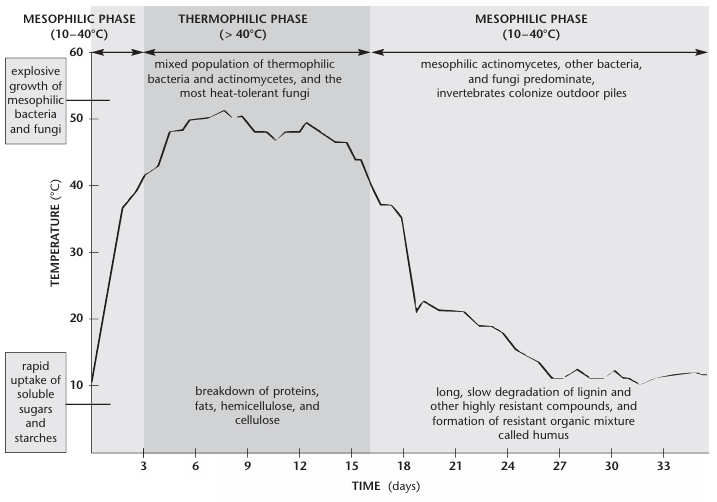
\includegraphics[scale=.7]{Figures/Compost Caracteristicas/Curva Temperatura.PNG}
	\caption{Curva característica de temperatura en una pila de compost \citep{curvaTemp}}
	\label{fig:curvatemp}
\end{figure}

\section{Estado Del Arte} % Main chapter title


\subsection{Estado del arte del compostaje en Argentina}
\label{sec:EstadoArteArgentina}

En Argentina, el compostaje se encuentra en una etapa inicial en cuanto a la adopción de tecnologías avanzadas para su monitoreo y control. La mayoría de las prácticas actuales son manuales y tradicionales y son muy pocos los organismos, entes o institutos que han adoptado alguna integración tecnológica (esto se debe principalmente por la falta de legislaciones en cuanto al tratamiento de residuos orgánicos).

\subsubsection{Desarrollos del INTA (Instituto Nacional de Tecnología Agropecuaria)}

El INTA trabajó hace unos años en una iniciativa donde se desarrollo un prototipo de sensores básicos para medir temperatura y humedad en compostajes rurales \footnote{Ver \url{https://intainforma.inta.gob.ar/desarrollan-sensor-para-optimizar-la-produccion-de-compost/}}. Sin embargo estos avances no han sidos implementados a nivel industrial o comercial hasta donde se ha podido investigar.

\subsubsection{Prácticas actuales}
A nivel industrial e individual, la mayoría de las maniobras relacionadas al compostaje se desarrollan de manera manual. Estas practicas incluyen:
\begin{itemize}
    \item Monitoreo de temperatura y humedad: la temperatura se miden empleando unos termómetros largos que se insertan en la pila de compost. Esta práctica se lleva a cabo varias veces por semana de manera de garantizar que el material en descomposición no alcance temperaturas críticas. Para la humedad se emplea el método del puño, que consiste en apretar una muestra de materia orgánica y observar si libera agua o se desmorona al soltarla.
    \item Volteo y aireación: en la mayoría de los casos, las pilas de compost son aireadas manualmente (por ejemplo mediante el uso de palas) o con maquinarias no especializadas (por ejemplo excavadoras).
\end{itemize}

Tal como se puede observar, las practicas actuales requieren la presencia de operarios en el lugar tanto sea para el monitoreo como para llevar a cabo acciones correctivas. Estas practicar aumentan la carga laboral y reducen la eficiencia del proceso; y exponen a un ambiente nocivo al operario en cuestión.

\subsection{Estado Del Arte del Compost a nivel global}
\label{sec:EstadoArteGlobal}

A nivel global las técnicas de compostaje han evolucionado significativamente y han surgido integraciones tecnológicas que permitieron optimizar el proceso, sobretodo en países con fuertes políticas de reciclaje y pioneros en innovación.
Se decidió detallar los casos de Estados Unidos y Japón para ejemplificar los avances a nivel global, ya que en otras partes del planeta y en países similares, los desarrollos se encuentran en fases similares.

\subsubsection{Estados Unidos}
En Estados Unidos existen soluciones privadas que integran IoT y automatizaciones para el monitoreo y procesamiento del compost. Dentro de ellas se destacan empresas como EcoRich \citep{ECORICH}

También destacan proyectos comunitarios, como el programa \textit{Zero Waste} \citep{ZeroWaste}, \textit{Farm Philly} \citep{FarmPhilly} y \textit{Denver Urban Gardens} \citep{DenverUrban}.

\subsubsection{Japón}
Entre las distintas tecnologías y proyectos comunitarios que Japón ha adoptado se destacan automatizaciones realizadas en colaboración con una empresa canadiense, \textit{Anaconda Systems Limited}\citep{Anaconda}, donde han desarrollado un sistema para compostar residuos orgánicos en cortos periodos de tiempo (aproximadamente 10 días).

A nivel gubernamental, Japón promueve el programa SATREP \textit{Science and Technology Research Partnership for Sustainable Development} \footnote{Ver \url{https://www.jst.go.jp/global/english/}}donde se hace énfasis en el manejo sostenible de residuos orgánicos.

\subsection{Conclusión}
El compostaje a nivel mundial se encuentra en un punto de desarrollo en el que, aunque existen avances tecnológicos notables, estos no son ni masivos ni altamente sofisticados en su implementación general. Los sistemas automatizados y las soluciones tecnológicas están presentes principalmente en países desarrollados como Estados Unidos, Japón y algunas naciones europeas, pero su adopción a gran escala es limitada. La mayoría de las prácticas siguen siendo manuales o dependen de métodos tradicionales, sobretodo en países en vías de desarrollo.

Se nota también que los proyectos comunitarios juegan un rol fundamental en la actividad del compostaje y que es de vital importancia la concientizacion social y el respaldo estatal.


\section{Alcance y Limitaciones}
Tal como se observa en la sección \ref{sec:CompostParámentros} son muchos los parámetros a tener en cuenta para obtener un compost de calidad. En este trabajo final se optó por medir temperatura y humedad debido a que según varios autores \citep{Risti} \citep{FactoresCompost} \citep{ManualBuenasPracticas} son los parámetros mas importantes y directos en cuanto a información del proceso se refiere y su medición es más simple y realizable que otros. Para ello se emplearon Nodos Sensores encargados de la medición, y Nodos \textit{Access Point} (AP) encargados de la distribución de la información medida.

Como base fundamental del trabajo se concluyo que el dispositivo SmartCompost es maniobrado por personal idóneo en el proceso de compostaje.

Se consideró que el dispositivo SmartCompost es empleado en zonas con red móvil, cualquiera sea el proveedor que exista en la región. 

No es necesaria la disponibilidad de energía eléctrica de red. La alimentación de los nodos sensores se da por baterías recargables y la alimentación de los Nodos AP con batería de ciclo profundo conectada a un panel solar que garantiza su recarga. En la sección \ref{ChapterDisenoImplementacion} se detalla mas información en cuanto a su funcionamiento.

La conectividad mediante los Nodos Sensores y el/los Nodo/s AP se resolvió mediante la tecnología LoRa, lo que permite cubrir áreas extensas de alrededor de 500 metros entre un Nodo Sensor y un Nodo AP.



No se consideró en el análisis la degradación de los sensores y su recalibración.


%----------------------------------------------------------------------------------------
%	SECCIÓN - REQUERIMIENTOS
%----------------------------------------------------------------------------------------

\section{Requerimientos} % Main chapter title

El desarrollo del proyecto SmartCompost se basó en un conjunto de requerimientos tanto funcionales como no funcionales, para garantizar que el sistema cumpla con las expectativas de rendimiento, facilidad de uso y sostenibilidad en el tiempo. 

\subsection{Requerimientos Funcionales}

\begin{itemize}
    \item \textbf{Monitoreo de temperatura y humedad}
    
    El sistema debe de monitorear de manera continua las condiciones de temperatura y humedad. Esto permite a los usuarios tomar decisiones informadas sobre el manejo de su compost.

    \item \textbf{Almacenamiento y análisis de datos}
    
    El sistema debe ser capaz de almacenar datos recolectados de los sensores  de manera eficiente y segura en una base de datos centralizada. Los datos deben ser almacenados en tiempo real y deben ser accesibles para su posterior análisis.

    \item \textbf{Autosuficiencia}
    
    El sistema debe operar de manera autónoma, minimizando la necesidad de intervención manual. Para ello debe contar con baterías recargables o paneles solares que garanticen su funcionamiento continuo.

    \item \textbf{Conectividad y transmisión}
    
    El sistema debe permitir la conectividad a través de diferentes protocolos de comunicación para la transmisión de datos, siendo compatible con tecnologías de comunicación inalámbricas como LoRa, WiFi, etc.

    \item \textbf{Interfaz de usuario sencilla}
    
    El sistema debe contener un componente para visualizar los datos en tiempo real de cada uno de los dispositivos. Esto incluye no solo las mediciones, sino la telemetría de los nodos. Debe requerir de la menor interacción del usuario para poder comprender la información.
    

\end{itemize}
\newpage

\subsection{Requerimientos No Funcionales}
\begin{itemize}
    \item \textbf{Durabilidad y resistencia}
    
    El sistema debe estar diseñado para operar en diversas condiciones ambientales y resistir factores externos que puedan afectar su funcionamiento.
    Debe soportar temperaturas extremas, variaciones de humedad y exposición a entornos hostiles.

    \item \textbf{Rendimiento y confiabilidad}
    
    El sistema debe funcionar de manera eficiente y confiable, asegurando la disponibilidad de datos precisos en todo momento.
    Debe implementar mecanismos de verificación de datos, como \textit{checksums} o validaciones, para asegurar la integridad de la información transmitida y almacenada.
    El sistema debe ser capaz de operar continuamente durante largos períodos sin interrupciones.

    \item \textbf{Escalabilidad}
    
    El sistema debe ser escalable para permitir la adición de nuevos sensores y funcionalidades en el futuro sin necesidad de reestructurar la infraestructura existente.
    Debe ser posible integrar nuevos dispositivos y sensores mediante protocolos estándar de comunicación sin afectar el rendimiento del sistema actual.

    \item \textbf{Facilidad de desarrollo y pruebas}

    El sistema debe ser fácil de desarrollar, optimizar y depurar. La integración de nuevos módulos no deben devenir en problemas de software ni debe agregar complejidad a la hora de compilar el proyecto. 

    \item \textbf{Portabilidad}
    
    El sistema debe ser fácil de transportar y reubicar en diferentes lugares según sea necesario. Para ello todos los componentes del sistema deben ser de tamaño compacto y ligero, facilitando el transporte y la instalación en diferentes ubicaciones.
    La estructura tiene que incluir soportes o carcasas que faciliten la instalación en diferentes entornos (como interiores o exteriores) y que puedan ser fijados de manera segura.
    La fuente de alimentación del sistema debe ser flexible, permitiendo su operación con diferentes fuentes de energía, sean baterías, energía solar o conexiones de red eléctrica.

    \item \textbf{Mantenibilidad}
    
    El sistema debe ser fácil de mantener y actualizar para garantizar su funcionalidad a lo largo del tiempo.
    Los componentes del sistema deben ser modulares, lo que permite su reemplazo o actualización sin afectar el resto del sistema.


\end{itemize}



% \chapter{Estado Del Arte} % Main chapter title

\label{Chapter2} % For referencing the chapter elsewhere, use \ref{Chapter1} 
\label{EstadoArte}


%----------------------------------------------------------------------------------------

%\section{Introducción}

%----------------------------------------------------------------------------------------
\section{Estado del arte del compostaje en Argentina}
\label{sec:EstadoArteArgentina}

En Argentina, el compostaje se encuentra en una etapa inicial en cuanto a la adopción de tecnologías avanzadas para su monitoreo y control. La mayoría de las prácticas actuales son manuales y tradicionales y son muy pocos los organismos, entes o institutos que han adoptado alguna integración tecnológica (esto se debe principalmente por la falta de legislaciones en cuanto al tratamiento de residuos orgánicos).

\subsection{Desarrollos del INTA (Instituto Nacional de Tecnología Agropecuaria)}

El INTA trabajó hace unos años en una iniciativa donde se desarrollo un prototipo de sensores básicos para medir temperatura y humedad en compostajes rurales \footnote{Ver \url{https://intainforma.inta.gob.ar/desarrollan-sensor-para-optimizar-la-produccion-de-compost/}}. Sin embargo estos avances no han sidos implementados a nivel industrial o comercial hasta donde se ha podido investigar.

\subsection{Prácticas actuales}
A nivel industrial e individual, la mayoría de las maniobras relacionadas al compostaje se desarrollan de manera manual. Estas practicas incluyen:
\begin{itemize}
    \item Monitoreo de temperatura y humedad: la temperatura se miden empleando unos termómetros largos que se insertan en la pila de compost. Esta práctica se lleva a cabo varias veces por semana de manera de garantizar que el material en descomposición no alcance temperaturas críticas. Para la humedad se emplea el método del puño, que consiste en apretar una muestra de materia orgánica y observar si libera agua o se desmorona al soltarla.
    \item Volteo y aireación: en la mayoría de los casos, las pilas de compost son aireadas manualmente (por ejemplo mediante el uso de palas) o con maquinarias no especializadas (por ejemplo excavadoras).
\end{itemize}

Tal como se puede observar, las practicas actuales requieren la presencia de operarios en el lugar tanto sea para el monitoreo como para llevar a cabo acciones correctivas. Estas practicar aumentan la carga laboral y reducen la eficiencia del proceso; y exponen a un ambiente nocivo al operario en cuestión.

\section{Estado Del Arte del Compost a nivel global}
\label{sec:EstadoArteGlobal}

A nivel global las técnicas de compostaje han evolucionado significativamente y han surgido integraciones tecnológicas que permitieron optimizar el proceso, sobretodo en países con fuertes políticas de reciclaje y pioneros en innovación.
Se decidió detallar los casos de Estados Unidos y Japón para ejemplificar los avances a nivel global, ya que en otras partes del planeta y en países similares, los desarrollos se encuentran en fases similares.

\subsection{Estados Unidos}
En Estados Unidos existen soluciones privadas que integran IoT y automatizaciones para el monitoreo y procesamiento del compost. Dentro de ellas se destacan empresas como EcoRich \citep{ECORICH}

También destacan proyectos comunitarios, como el programa \textit{Zero Waste} \citep{ZeroWaste}, \textit{Farm Philly} \citep{FarmPhilly} y \textit{Denver Urban Gardens} \citep{DenverUrban}.

\subsection{Japón}
Entre las distintas tecnologías y proyectos comunitarios que Japón ha adoptado se destacan automatizaciones realizadas en colaboración con una empresa canadiense, \textit{Anaconda Systems Limited}\citep{Anaconda}, donde han desarrollado un sistema para compostar residuos orgánicos en cortos periodos de tiempo (aproximadamente 10 días).

A nivel gubernamental, Japón promueve el programa SATREP \textit{Science and Technology Research Partnership for Sustainable Development} \footnote{Ver \url{https://www.jst.go.jp/global/english/}}donde se hace énfasis en el manejo sostenible de residuos orgánicos.

\section{Conclusión}
El compostaje a nivel mundial se encuentra en un punto de desarrollo en el que, aunque existen avances tecnológicos notables, estos no son ni masivos ni altamente sofisticados en su implementación general. Los sistemas automatizados y las soluciones tecnológicas están presentes principalmente en países desarrollados como Estados Unidos, Japón y algunas naciones europeas, pero su adopción a gran escala es limitada. La mayoría de las prácticas siguen siendo manuales o dependen de métodos tradicionales, sobretodo en países en vías de desarrollo.

Se nota también que los proyectos comunitarios juegan un rol fundamental en la actividad del compostaje y que es de vital importancia la concientizacion social y el respaldo estatal.




% \chapter{Requerimientos} % Main chapter title

\label{Chapter3}

%----------------------------------------------------------------------------------------
%	SECCIÓN - REQUERIMIENTOS
%----------------------------------------------------------------------------------------

El desarrollo del proyecto SmartCompost se basó en un conjunto de requerimientos tanto funcionales como no funcionales, para garantizar que el sistema cumpla con las expectativas de rendimiento, facilidad de uso y sostenibilidad en el tiempo. 

\section{Requerimientos Funcionales}

\begin{itemize}
    \item \textbf{Monitoreo de temperatura y humedad}
    
    El sistema debe de monitorear de manera continua las condiciones de temperatura y humedad. Esto permite a los usuarios tomar decisiones informadas sobre el manejo de su compost.

    \item \textbf{Almacenamiento y análisis de datos}
    
    El sistema debe ser capaz de almacenar datos recolectados de los sensores  de manera eficiente y segura en una base de datos centralizada. Los datos deben ser almacenados en tiempo real y deben ser accesibles para su posterior análisis.

    \item \textbf{Autosuficiencia}
    
    El sistema debe operar de manera autónoma, minimizando la necesidad de intervención manual. Para ello debe contar con baterías recargables o paneles solares que garanticen su funcionamiento continuo.

    \item \textbf{Conectividad y transmisión}
    
    El sistema debe permitir la conectividad a través de diferentes protocolos de comunicación para la transmisión de datos, siendo compatible con tecnologías de comunicación inalámbricas como LoRa, WiFi, etc.

    \item \textbf{Interfaz de usuario sencilla}
    
    El sistema debe contener un componente para visualizar los datos en tiempo real de cada uno de los dispositivos. Esto incluye no solo las mediciones, sino la telemetría de los nodos. Debe requerir de la menor interacción del usuario para poder comprender la información.
    

\end{itemize}
\newpage

\section{Requerimientos No Funcionales}
\begin{itemize}
    \item \textbf{Durabilidad y resistencia}
    
    El sistema debe estar diseñado para operar en diversas condiciones ambientales y resistir factores externos que puedan afectar su funcionamiento.
    Debe soportar temperaturas extremas, variaciones de humedad y exposición a entornos hostiles.

    \item \textbf{Rendimiento y confiabilidad}
    
    El sistema debe funcionar de manera eficiente y confiable, asegurando la disponibilidad de datos precisos en todo momento.
    Debe implementar mecanismos de verificación de datos, como \textit{checksums} o validaciones, para asegurar la integridad de la información transmitida y almacenada.
    El sistema debe ser capaz de operar continuamente durante largos períodos sin interrupciones.

    \item \textbf{Escalabilidad}
    
    El sistema debe ser escalable para permitir la adición de nuevos sensores y funcionalidades en el futuro sin necesidad de reestructurar la infraestructura existente.
    Debe ser posible integrar nuevos dispositivos y sensores mediante protocolos estándar de comunicación sin afectar el rendimiento del sistema actual.

    \item \textbf{Facilidad de desarrollo y pruebas}

    El sistema debe ser fácil de desarrollar, optimizar y depurar. La integración de nuevos módulos no deben devenir en problemas de software ni debe agregar complejidad a la hora de compilar el proyecto. 

    \item \textbf{Portabilidad}
    
    El sistema debe ser fácil de transportar y reubicar en diferentes lugares según sea necesario. Para ello todos los componentes del sistema deben ser de tamaño compacto y ligero, facilitando el transporte y la instalación en diferentes ubicaciones.
    La estructura tiene que incluir soportes o carcasas que faciliten la instalación en diferentes entornos (como interiores o exteriores) y que puedan ser fijados de manera segura.
    La fuente de alimentación del sistema debe ser flexible, permitiendo su operación con diferentes fuentes de energía, sean baterías, energía solar o conexiones de red eléctrica.

    \item \textbf{Mantenibilidad}
    
    El sistema debe ser fácil de mantener y actualizar para garantizar su funcionalidad a lo largo del tiempo.
    Los componentes del sistema deben ser modulares, lo que permite su reemplazo o actualización sin afectar el resto del sistema.


\end{itemize}

 
\include{Chapters/Chapter4-DiseñoImplementacion}
% Chapter Template

\chapter{Ensayos y resultados} % Main chapter title

\label{Chapter5} 


%----------------------------------------------------------------------------------------
%	SECTION - PRUEBAS FUNCIONALES
%----------------------------------------------------------------------------------------
\section{Pruebas funcionales}
\label{sec:pruebas}
En esta sección se mencionan las pruebas funcionales unitarias realizadas sobre los diferentes puntos del proyecto.

%----------------------------------------------------------------------------------------
%	SUBSECTION - PRUEBAS FUNCIONALES DEL HARDWARE
%----------------------------------------------------------------------------------------
\subsection{Pruebas funcionales del hardware}
\label{sec:pruebasHW}

\subsubsection{Sensor temperatura DS18B20}
En esta sección se describe el banco de pruebas utilizado y la conexión del sensor DS18B20 al microcontrolador ESP32, detallando su configuración eléctrica y las consideraciones de hardware necesarias.

\subsubsection{Banco de pruebas}
Para realizar las pruebas se utilizaron los siguientes componentes:
\begin{itemize}
    \item Sensor de temperatura DS18B20.
    \item Placa de desarrollo ESP32.
    \item Resistencia de 4.7k$\Omega$.
    \item Cables de conexión.
    \item \textit{Protoboard}.
\end{itemize}

\subsubsection{Conexión del Sensor DS18B20 a la ESP32}
El DS18B20 tiene tres pines: VCC, GND y DATA. El pin DATA utiliza un protocolo 1-Wire para la comunicación con la ESP32, por lo que solo necesita un pin de entrada/salida en el PCB. La conexión se realizó de la siguiente manera:

\begin{itemize}
    \item VCC del DS18B20 conectado a 5 V.
    \item GND del DS18B20 conectado a GND .
    \item DATA del DS18B20 conectado al pin GPIO17 de la ESP32.
    \item Se utilizó una resistencia de 4.7k$\Omega$ entre VCC y el pin DATA para asegurar la correcta comunicación, tal como lo indica la hoja de datos del fabricante \citep{Sensor_temp}.
\end{itemize}

La figura \ref{fig:conexionTemperatura} muestra el diagrama de conexión del sensor DS18B20 a la ESP32.

\begin{figure}[h]
    \centering
    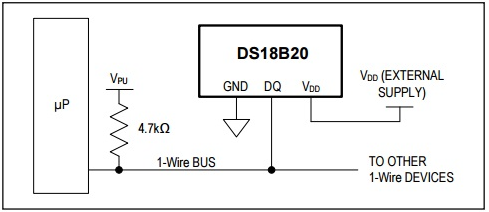
\includegraphics[width=0.8\textwidth]{./Figures/Pruebas/conexion_ds18b20.png}
    \caption{Conexión del sensor DS18B20 a la ESP32.}
    \label{fig:conexionTemperatura}
\end{figure}

\subsubsection{Código Implementado}
El código se escribió utilizando el entorno de desarrollo VisualStudio 2022, con la biblioteca nanoFramework.Device.OneWire para la comunicación del sensor y la biblioteca Iot.Device.Ds18b20 para la lectura de los datos de temperatura. El siguiente fragmento de código \ref{codigoDS18B20} se empleo para el desarrollo de la prueba:
\begin{lstlisting}[language=C, label=codigoDS18B20, caption= Fragmento del código del sensor de temperatura DS18B20]

using Iot.Device.Ds18b20;
using nanoFramework.Device.OneWire;

        private void ConfigurarSensorTemperatura()
        {
            Configuration.SetPinFunction(16, DeviceFunction.COM3_RX);
            Configuration.SetPinFunction(17, DeviceFunction.COM3_TX);

            OneWireHost oneWire = new OneWireHost();


            ds18b20 = new Ds18b20(oneWire, null, false, TemperatureResolution.VeryHigh);

            ds18b20.IsAlarmSearchCommandEnabled = false;
            if (ds18b20.Initialize())
            {
                Console.WriteLine($"Is sensor parasite powered?:{ds18b20.IsParasitePowered}");
                string devAddrStr = "";
                foreach (var addrByte in ds18b20.Address)
                {
                    devAddrStr += addrByte.ToString("X2");
                }

                Console.WriteLine($"Sensor address:{devAddrStr}");
            }
        }

                private double MedirTemperatura()
        {
            if (!ds18b20.TryReadTemperature(out var currentTemperature))
            {
                Console.WriteLine("Can't read!");
                return -1;
            }
            else
            {
                Console.WriteLine($"Temperature: {currentTemperature.DegreesCelsius.ToString("F")}\u00B0C");
                return currentTemperature.DegreesCelsius;
            }
        }
\end{lstlisting}

\subsubsection{Resultados de las Pruebas}
Las pruebas se realizaron en condiciones de laboratorio. Para ello se introdujo el sensor en una maceta con tierra y arena (simulando las condiciones de trabajo real) y se agregó agua caliente para variar la temperatura del suelo. Se usó un termómetro digital para comparar las lecturas de temperatura \citep{Magesa} y validar el funcionamiento del sensor de temperatura DS18B20.

Se observaron los siguientes resultados:
\begin{itemize}
    \item El sensor DS18B20 se conectó exitosamente a la placa ESP32, siguiendo el esquema de conexión descrito.
    \item La comunicación entre el sensor y la ESP32 fue estable gracias a la resistencia de pull-up de 4.7k$\Omega$ entre VCC y DATA.
    \item Las lecturas de temperatura fueron consistentes y precisas en un rango de 10°C a 80°C, mostrando una precisión dentro de ±0.5°C, que es lo esperado para este sensor.
    \item Los resultados se imprimieron en el monitor serial, actualizándose cada segundo.
    \item Las condiciones de humedad no afectaron ni destruyeron al sensor, comprobando su capacidad de sumergible.
\end{itemize}

\subsubsection{Conclusiones}
El sensor de temperatura DS18B20 es una solución efectiva para medir temperaturas con precisión y simplicidad, utilizando una única línea de datos para la comunicación con la ESP32. Las pruebas realizadas confirmaron el correcto funcionamiento del sistema, con resultados precisos y consistentes.


\subsubsection{Sensor de Humedad YL-69}
A continuación se describen la conexión y pruebas realizadas con el sensor de humedad YL-69, que se utiliza para medir la humedad del suelo.

\subsubsection{Banco de pruebas}
Para realizar las pruebas se utilizaron los siguientes componentes:
\begin{itemize}
    \item Sensor de humedad YL-69.
    \item Módulo comparador YL-38.
    \item Placa de desarrollo ESP32.
    \item Cables de conexión.
    \item Protoboard.
    \item Fuente de alimentación de 5 V.
\end{itemize}

\subsubsection{Conexión del Sensor de Humedad YL-69 a la ESP32}
El sensor de humedad YL-69 es un dispositivo que mide la resistencia entre dos sondas insertadas en el suelo. Esta medición se traduce en un valor analógico que refleja la humedad del suelo. El sensor YL-69 funciona junto con el módulo YL-38, que convierte la señal analógica en digital para facilitar la lectura con microcontroladores.

La conexión se realizó de la siguiente manera:

\begin{itemize}
    \item VCC del YL-38 conectado a 5 V.
    \item GND del YL-38 conectado a GND.
    \item La salida analógica (A0) del YL-38 conectada al pin GPIO35 (entrada ADC) de la ESP32.
    \item Las sondas del YL-69 conectadas a los pines correspondientes del módulo YL-38.
\end{itemize}

La Figura \ref{fig:conexion_yl69} muestra el diagrama de conexión del sensor de humedad YL-69 al ESP32.

\begin{figure}[h]
    \centering
    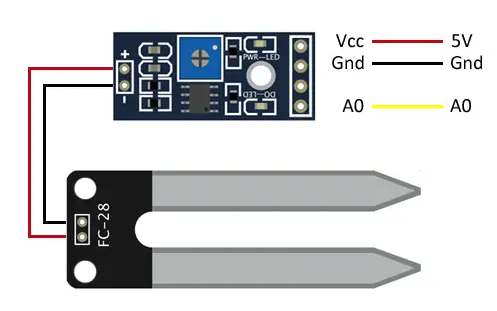
\includegraphics[width=0.8\textwidth]{./Figures/Pruebas/conexion_yl69.png}
    \caption{Conexión del sensor de humedad YL-69 al ESP32. Fuente: \citep{higrometroFC-28}.}
    \label{fig:conexion_yl69}
\end{figure}

\subsubsection{Código Implementado}
El código se escribió utilizando el mismo entorno de desarrollo que para el sensor de temperatura. El valor analógico del sensor de humedad se lee a través del puerto ADC de la ESP32.

El fragmento de código \ref{codigoYL-69} se utilizo para realizar las pruebas correspondientes.

\begin{lstlisting}[language=C, label=codigoYL-69, caption= Fragmento del código del sensor de humedad YL-69]

using System;
using nanoFramework.Hardware.Esp32;
using Windows.Devices.Adc;

        private void ConfigurarSensorHumedad()
        {
            // Configurar el pin ADC
            adc = new AdcController();

            //HUMEDAD          -----> ADC Channel 7 - GPIO 35 
            humedadAdc = adc.OpenChannel(7);

            Console.WriteLine("Sensor de humedad configurado.");
        }

         private double MedirHumedad()
        {
            
            
            int analogValue = humedadAdc.ReadValue();

            float vSensor = (analogValue / 4095f * 3.3f);
            double humidityPercentage = (-48.95 * vSensor * vSensor * vSensor) + (368.10 * vSensor * vSensor) - 910.85 * vSensor + 757.17;

            Console.WriteLine($"Analog Humedad: {analogValue}");
            Console.WriteLine($" tension: {vSensor}");
            if(humidityPercentage>100) humidityPercentage=100;
            if(humidityPercentage<0) humidityPercentage=0;

            return humidityPercentage;

        }
\end{lstlisting}

Es importante destacar que la humedad del suelo es un parámetro relativo ya que no se mide en términos absolutos (litros de agua por metro cúbico de suelo) en la mayoría de los casos, sino en relación a la capacidad del suelo para retener agua. Hay varios parámetros clave que hacen de la humedad del suelo una medida relativa, como por ejemplo la temperatura y la presión.

Es por eso que para la calibración del sensor de humedad se tuvo en cuenta un estudio\cite{yl_69_calibration} donde se comparó las mediciones del sensor con las de un método más preciso conocido como el método gravimétrico.

Con los resultados de este estudio se desarrollaron mediciones comparativas y aproximaciones polinómicas de las lecturas del ADC para obtener una fórmula que permita traducir los niveles de tensión a porcentaje de humedad. Esto dió como resultado la siguiente fórmula:

\begin{equation}
f(x) = 757.17 - 910.85x + 368.01x^2 - 48.95x^3
\end{equation}


\subsubsection{Resultados de las Pruebas}
Las pruebas se realizaron insertando las sondas del sensor YL-69 en diferentes tipos de suelos, desde secos hasta saturados de agua. Se realizaron varias mediciones y se observaron los siguientes resultados:

\begin{itemize}
    \item El sensor YL-69 se conectó exitosamente a la ESP32, y las lecturas de humedad se obtuvieron sin inconvenientes.
    \item El sensor respondió de manera eficiente a los cambios en el nivel de humedad del suelo, mostrando un aumento en los valores analógicos a medida que el suelo se humedecía.
    \item Las lecturas variaron entre un 0\% de humedad en suelo seco hasta un 100\% en suelo saturado.
    \item La estabilidad de las lecturas se mantuvo, incluso en condiciones de humedad extrema.
\end{itemize}

\subsubsection{Conclusiones}
Es importante mencionar que normalmente la manera de medir la humedad del compost se desarrolla de manera manual, tomando una cierta cantidad de compost en las manos y comprimiéndola para ver si drena agua entre los dedos y se forma una masa barrosa, o si al soltarlo el material se desparrama.

El sensor de humedad YL-69 demostró ser un instrumento eficaz para medir la humedad del suelo, proporcionando lecturas confiables en un rango amplio de condiciones. La integración con la ESP32 fue sencilla, y el uso del módulo YL-38 permitió leer tanto señales digitales como analógicas del sensor. Los resultados obtenidos en las pruebas indicaron un comportamiento estable y preciso. El método diseñado para medir la humedad permite reemplazar el trabajo manual y proveer un poco más de información sin estar presente en la zona.



\subsubsection{Panel Solar Cargador Batería 12 V 10 W}
A continuación, se describen las conexiones y pruebas realizadas con el panel solar Cargador Batería 12 V 10 W.

\subsubsection{Banco de pruebas}
Para realizar este proyecto, se utilizaron los siguientes componentes:
\begin{itemize}
    \item Panel  Solar Cargador Batería 12 V 10 W.
    \item Controlador de carga solar.
    \item Batería de 12 V.
    \item Cables de conexión.
    \item Multímetro.
\end{itemize}

\subsubsection{Conexión del Panel Solar a la Batería}
El panel Solar Cargador Batería 12 V 10 W se utilizó para cargar una batería de 12 V mediante un controlador de carga solar. La conexión se realizó de la siguiente manera:

\begin{itemize}
    \item Conectar el terminal positivo del panel solar al terminal positivo de la entrada del controlador de carga.
    \item Conectar el terminal negativo del panel solar al terminal negativo de la entrada del controlador de carga.
    \item Conectar el terminal positivo de la batería al terminal positivo de la salida del controlador de carga.
    \item Conectar el terminal negativo de la batería al terminal negativo de la salida del controlador de carga.
\end{itemize}

La Figura \ref{fig:conexionPanel} muestra el diagrama de conexión del panel solar al controlador de carga y a la batería.

\begin{figure}[h]
    \centering
    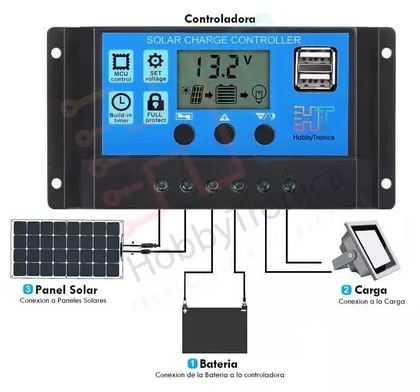
\includegraphics[width=0.8\textwidth]{./Figures/Pruebas/conexion_panel_solar.png}
    \caption{Conexión del panel Solar Cargador Batería 12 V 10 W.}
    \label{fig:conexionPanel}
\end{figure}


\subsubsection{Resultados de las Pruebas}
Las pruebas se realizaron en condiciones de iluminación natural, colocando el panel solar al aire libre. A continuación, se detallan los resultados:

\begin{itemize}
    \item El panel solar fue capaz de generar un voltaje constante en condiciones de sol pleno, alcanzando aproximadamente 14.5 V.
    \item El controlador de carga funcionó adecuadamente, regulando el voltaje y protegiendo la batería de sobrecargas.
    \item La batería se cargó satisfactoriamente, manteniendo un voltaje de alrededor de 13.8 V al finalizar la prueba.
\end{itemize}

\subsubsection{Conclusiones}
El panel solar Solar Cargador Batería 12 V 10 W es una solución adecuada para la carga de baterías de 12 V en sistemas de baja potencia. Las pruebas realizadas confirmaron su capacidad de generar energía suficiente bajo condiciones de sol pleno. Además, la integración con un controlador de carga garantiza la protección de la batería y una carga eficiente, logrando resultados estables y predecibles.

\subsection{Cálculos de alimentación Nodo Sensor}
\subsubsection{Consumos Nodo Sensor}
Para estimar el consumo y la duración de las baterías del Nodo Sensor, se buscó en las hojas de datos el consumo máximo de cada componente del sistema y se calculó el consumo total del nodo. 

En la tabla \ref{tab:consumosNodo} se notan estos valores (el consumo total se indican en mas de un renglón pero con distintas unidades).


\begin{table}[h]
    \centering

    \begin{tabular}{@{}lc@{}}
        \toprule
        \textbf{Componente}            & \textbf{Consumo (mA)} \\ \midrule
        ESP32 Wroom                   & 120 mA (promedio)      \\ 
        LoRa SX1278                   & 120 mA                  \\ 
        Sensor de temperatura DS18B20  & 1,5 mA     \\ 
        Sensor de humedad YL-69        & 20 mA                  \\ 
        Regulador Mini-360             & 90\% eficiencia                  \\ \midrule
        %\textbf{Consumo total}        & \textbf{287.65 mA}     \\ \bottomrule
        \textbf{Consumo total}        & \textbf{1438 mW}     \\ \bottomrule
    \end{tabular}
    \caption{Consumo de los componentes en mAh}
    \label{tab:consumosNodo}
\end{table}

\subsubsection{Capacidad de la pilas}
En la tabla \ref{tab:capacidadPilas} se denota la capacidad de las pilas. Para el cálculo de la capacidad efectiva de las pilas se tuvo en cuenta el nivel de tensión mínimo que el fabricante recomienda (ver sección \ref{sec:AlimentacionNodoSensor}). 

Al realizar el cálculo:
\begin{equation}
   \frac{Tension_{min} * Capacidad (Ah)}{Tension_{max}} = \frac{5.6v * 3.5Ah}{7.5v} = 2.61 Ah
\label{eq:capacidadEfectiva}
\end{equation}

Se obtiene la capacidad efectiva en Ah. Al multiplicar este valor por el valor de la tensión mínima, se obtiene la capacidad en Wh, siendo esta de 14.63 Wh.

Por último, al final de la tabla \ref{tab:capacidadPilas} se nota el tiempo de funcionamiento en horas del sistema en un régimen de trabajo de modo continuo.

\begin{table}[H]
    \centering
    \begin{tabular}{@{}lc@{}}
        \toprule
        \textbf{Especificación}       & \textbf{Valor}          \\ \midrule
       % Capacidad de las pilas      & 3.5 Ah (3500 mAh)        \\ 
        Capacidad de las pilas     & 25,9 Wh       \\ 
       % Capacidad efectiva de las pilas (Ah)      & 2,613 Ah      \\ 
        Capacidad efectiva de las pilas      & 14,63 Wh      \\ 
        Tiempo de funcionamiento & $\frac{14,63 \text{ Wh}}{1,43 \text{ w}} \approx 10,17 \text{ horas}$ \\ \bottomrule
    \end{tabular}
    \caption{Capacidad de las pilas}
    \label{tab:capacidadPilas}
\end{table}

A modo de prueba se decidió por implementar un régimen de trabajo de envío de información cada 10 segundos. Es decir, el sistema realiza una medición, envía la información sensada al Nodo AP y únicamente el ESP32 y el LoRa entran en modo Deep Sleep durante los próximos 10 segundos. Tanto los sensores de temperatura y humedad como el regulador de tensión permanecen con sus regímenes de consumo normal.

Bajo este régimen de trabajo, el sistema duró aproximadamente 21 horas operando, tal como lo indica la figura \ref{fig:PruebaBateria}.

\subsubsection{Conclusión}
Considerando que el régimen de trabajo normal es una medición por hora, es decir, una frecuencia de trabajo 360 veces más lenta que la sometida a prueba, y realizando una estimación general, se calcula que la autonomía del sistema sería aproximadamente de 7560 horas, lo que equivale a 315 días.

Teniendo en cuenta que el proceso de descomposición de la materia orgánica suele durar entre 3 y 5 meses aproximadamente (dependiendo de varios factores, como por ejemplo estación del año), se contempla que la autonomía de la batería es más que suficiente y cumple los requisitos establecidos.

\begin{figure}[H]
	\centering
	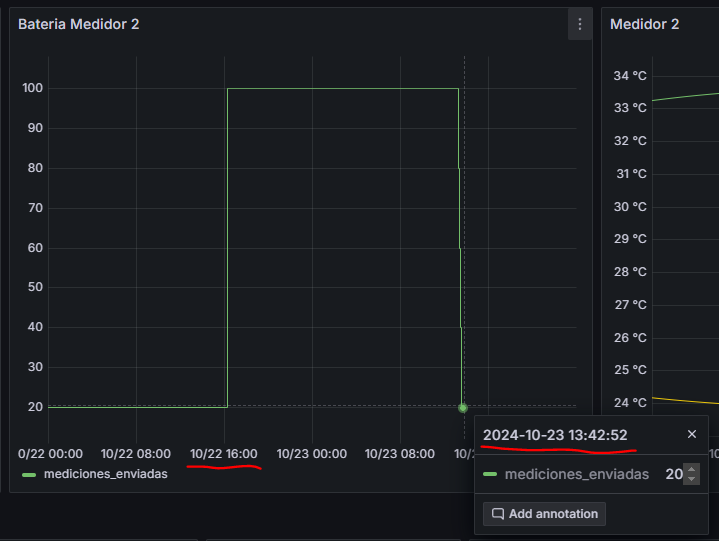
\includegraphics[scale=0.9]{./Figures/Pruebas/duracion_pila.png}
	\caption{Duración pilas - régimen de trabajo : 10 sg}
	\label{fig:PruebaBateria}
\end{figure}



\subsection{Cálculos de alimentación Nodo Access Point}
\subsubsection{Consumos componentes Nodo Access Point}

Para estimar el consumo y la duración de la batería del Nodo Access Point, se consultaron las hojas de datos para obtener el consumo máximo de cada componente del sistema y se calculó el consumo total del nodo. En la Tabla \ref{tab:consumosAP} se detallan estos valores.

\begin{table}[H]
    \centering

    \begin{tabular}{@{}lc@{}}
        \toprule
        \textbf{Componente}            & \textbf{Consumo (mA)} \\ \midrule
        ESP32 Wroom                   & 120 mA (promedio)      \\ 
        LoRa SX1278                   & 10.8 mA                  \\ 
        Router 4G portátil            & 300 mA                  \\ 
        Gerenciador                 & 10 mA                  \\ 
        Regulador Mini-360             & 90\% eficiencia                  \\ \midrule
     %   \textbf{Consumo total}        & \textbf{454 mA}     \\ \bottomrule
        \textbf{Consumo total}        & \textbf{2270 mW}     \\ \bottomrule
    \end{tabular}
    \caption{Consumo de los componentes en mAh}
    \label{tab:consumosAP}
\end{table}

Se observa una diferencia en los valores del modulo LoRa, ya que para este nodo el funcionamiento del modulo es en modo escucha y no en transmisión.

\subsubsection{Capacidad de la batería}
En la tabla \ref{tab:capacidadBat} se muestra la capacidad de la batería. Para calcular la capacidad efectiva de la batería se tomó en cuenta el nivel de tensión mínima recomendado por el fabricante. Se empleó la cuenta \ref{eq:capacidadEfectiva} dando como resultado una capacidad efectiva de 58.33 Wh.
Por último se nota que el tiempo de funcionamiento en modo continuo es de aproximadamente 25.7 horas.
\begin{table}[H]
    \centering
    \begin{tabular}{@{}lc@{}}
        \toprule
        \textbf{Especificación}       & \textbf{Valor}          \\ \midrule
       % Capacidad de la batería       & 7 Ah (7000 mAh)        \\ 
        Capacidad de la batería       & 84 Wh       \\ 
      %  Capacidad efectiva de la batería       & 5,83 Ah      \\ 
        Capacidad efectiva de la batería       & 58.33 Wh      \\ 
        Tiempo de funcionamiento  & $\frac{58.3 \text{ Wh}}{2.27 \text{ w}} \approx 25.7 \text{ horas}$ \\ \bottomrule
    \end{tabular}
    \caption{Capacidad de las baterías del Nodo Access Point}
    \label{tab:capacidadBat}
\end{table}
Para realizar la prueba de autonomía se establecieron las siguientes configuraciones:

\begin{itemize}
    \item La batería se encontraba cargada al 100\%.
    \item Se desconecto el panel solar para evitar cargar la batería.
    \item Se estableció una frecuencia de envió de métricas del Nodo Access Point al portal de 5 mins.
    \item Se estableció una frecuencia de envío de métricas del Nodo Sensor al Nodo Access Point de 10 segundos.
\end{itemize}
Bajo estas condiciones de trabajo, la autonomía del Nodo Access Point fue de 23 horas.

\subsubsection{Conclusión}
Considerando que el régimen de trabajo normal es una medición por hora y que el panel solar se encuentra conectado al sistema (aportando carga a la batería), se contempla que la autonomía de la batería es suficiente y cumple los requisitos establecidos, aunque como mejora del sistema se podría optar por una batería de una capacidad un poco mayor para tener mas autonomía. 
%----------------------------------------------------------------------------------------
%	SUBSECTION - PRUEBAS FUNCIONALES DEL FIRMWARE
%----------------------------------------------------------------------------------------
\subsection{Pruebas funcionales del firmware}
\label{sec:pruebasFW}

El objetivo de estas pruebas era determinar el correcto funcionamiento del firmware, tanto del NanoKernel, como de los Nodos Sensor y Nodo Access Point. 
Para ello se armaron pruebas incrementales, de forma tal de primero probar funcionalidades unitarias, y luego hacer pruebas integrales en un entorno local y controlado (sin uso del portal web).

Para todas estas pruebas, se utilizaron las herramientas de debugging nativas de Visual Studio 22 y la extensión de nanoframework, como también herramientas de logging en servicios web locales, y mediciones del espectro en la banda de transmisión de LoRa.

\subsubsection{Listado de pruebas}

Las pruebas fueron las siguientes:

\begin{enumerate}
    \item Correcto funcionamiento del NanoKernel.
    \item Conectividad a red Wi-Fi desde un nodo.
    \item Conexión y envío de paquetes LoRa desde un nodo.
    \item Envió de paquetes LoRa desde un nodo hacia otro.
    \item Prueba de envío de un \textit{payload} JSON desde un nodo a un servicio web en una red WiFi local.
    \item Prueba de Nodo Sensor con medición de sensores, envío de paquete LoRa, y bucle con DeepSleep.
    \item Prueba de Nodo Access Point  con simulación de paquetes LoRa entrante, manejo de colas, y envío de mediciones a servicio web en red local.
    \item Prueba de Nodo Sensor y Nodo Access Point, contra un servicio web en red local.
    \item Prueba de 2 Nodo Sensor y Nodo Access Point, contra un servicio web en red local.
    \item Prueba final de 2 Nodo Sensor y Nodo Access Point, conectados al router 4G portátil, contra un servicio en la red local expuesto a la red pública.
\end{enumerate}

Una vez realizada la prueba 10, se considera que el firmware se encuentra en condiciones de acoplarse al sistema del Portal web: como todas las pruebas se realizaron teniendo en cuenta el contrato de servicios establecido por el Portal web, la integración real consiste en simplemente un cambio de url en el endpoint.

\subsubsection{Resultados}

Entre los principales desafíos de las pruebas se encuentra el manejo de la tecnología LoRa, ya que la misma implica distintas dificultades tanto a nivel hardware como firmware.
Es por eso que para la prueba 3 no sólo se hizo uso de logeo en depuración, sino tambien de un analizador de espectro digital (SDR basado en el chip rtl2832u) para poder depurar la señal, confirmar la frecuencia de su portadora, ancho de banda, y nivel respecto al piso de ruido. Para ello se empleó la herramienta AirSpy, el cual permite observar el espectro en base al IQ enviado por USB del SDR, como se observa en la figura \ref{fig:pruebas_firmware_1}.

\begin{figure}[H]
    \centering
    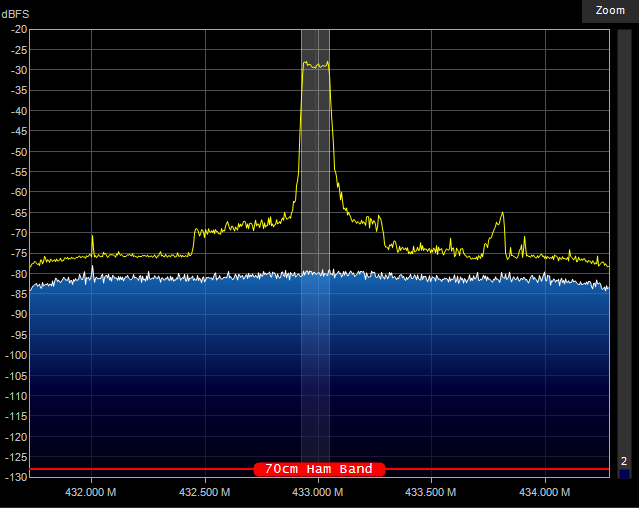
\includegraphics[width=1\linewidth]{Figures/Firmware/espectro.png}
    \caption{Análisis espectral de un emisor LoRa con la portadora en 433 MHz y 125 kHz de ancho de banda.}
    \label{fig:pruebas_firmware_1}
\end{figure}

Con esta herramienta se permitió determinar, no sólo que efectivamente el Módulo LoRa está enviando paquetes en el medio, sino también corroborar su correcta configuración de portadora y ancho de banda (entre otros). Esto es así ya que el umbral amarillo (detector de máximos) muestra que la señal LoRa se encuentra ubicada correctamente en la portadora de 433 MHz, con un ancho de banda de 125 KHz, y un nivel de la señal sobre el piso de ruido (SNR) mucho mayor a 0dB. Éste último parámetro es de vital importancia ya que indica la calidad con la que el receptor va a recibir la señal. Depende principalmente de la corriente que pueda brindar la fuente de alimentación, de la antena del Módulo LoRa, la antena del SDR, y la distancia entre las antenas. En este caso, dado que no hace falta una medición espectral absoluta ni precisa, simplemente de forma preliminar se puede observar que el Módulo LoRa opera en rangos correctos.

Por otra parte, otro de los obstáculos que se encontraron a lo largo de las pruebas fue el manejo de memoria por parte del Nodo Access Point, ya que el mismo almacena en un \textit{buffer} los mensajes encolados para enviar, por lo que es un recurso muy limitado que sobrecargaba al \textit{garbage collector}, y por ende a la CPU.

Dado que todas las pruebas se realizaron en modo depuración, fue de vital importancia tener registro de la memoria total, memoria liberada, cantidad de paquetes encolados, paquetes enviados, paquetes perdidos, la cantidad de errores, etc, y así poder describir al sistema con el fin de parametrizar la configuración y conseguir el mayor throughput con la menor tasa de error posible. En la Figura \ref{fig:pruebas_firmware_2} se observa un extracto de los logs del Nodo AP:

\begin{figure}[H]
    \centering
    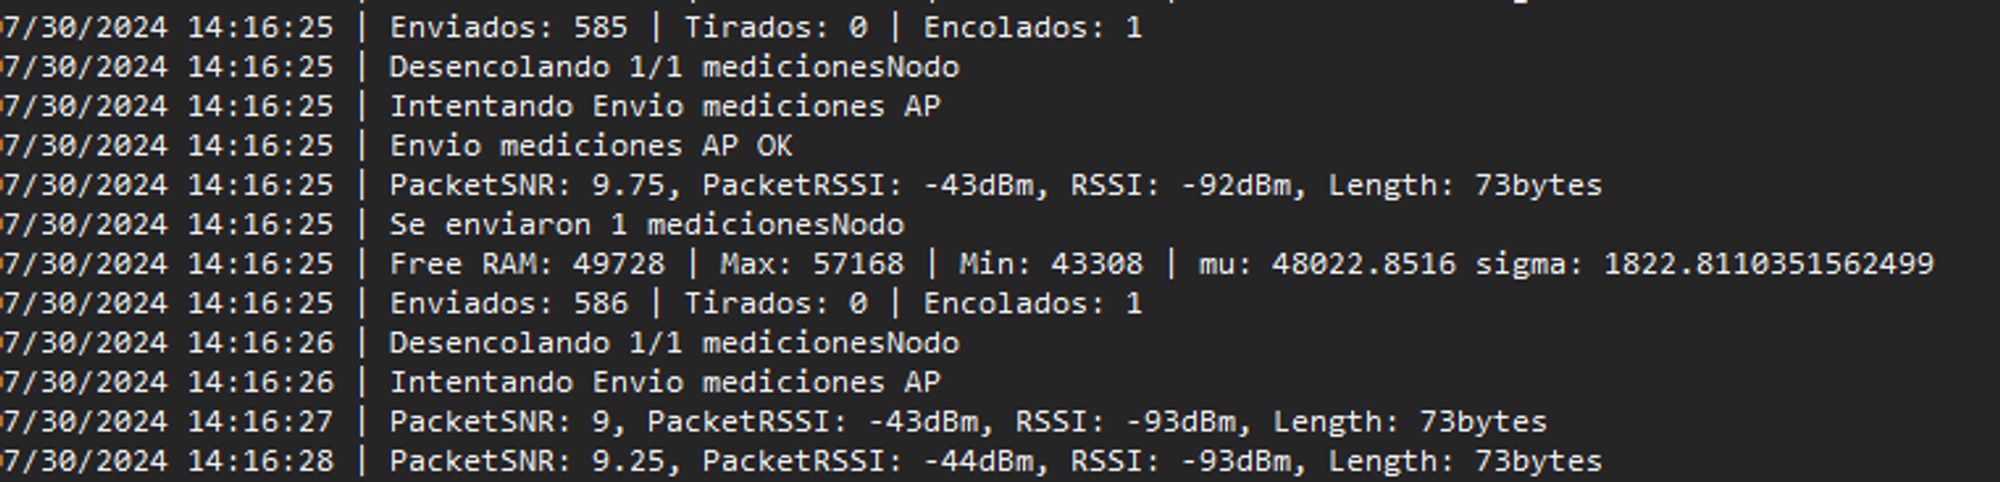
\includegraphics[width=1\linewidth]{Figures/Firmware/pruebas_2.png}
    \caption{Ejemplo captura de logging del Nodo Access Point.}
    \label{fig:pruebas_firmware_2}
\end{figure}

Para el monitoreo de memoria y cuantización de paquetes y errores se utilizó una herramienta ad hoc de muestreo de valores, el cual registra la cantidad de mediciones, el máximo, mínimo, promedio y desvío estándar.

\begin{figure}[H]
    \centering
    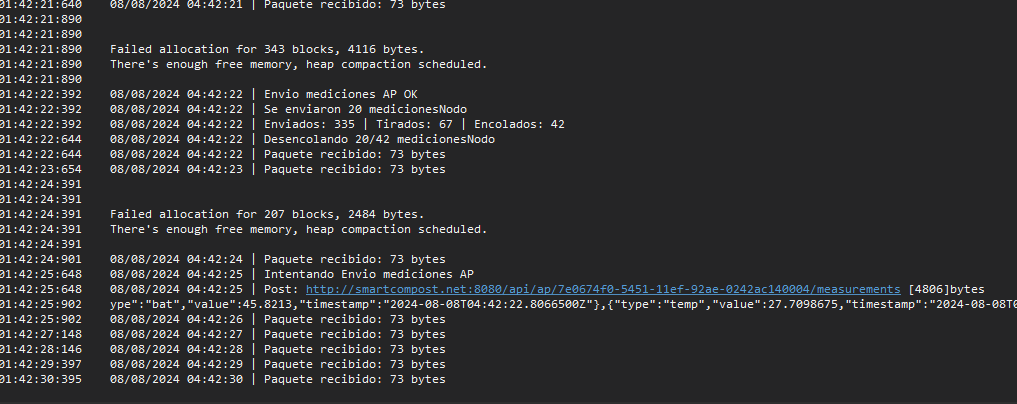
\includegraphics[width=1\linewidth]{Figures/Firmware/pruebas_1.png}
    \caption{Captura de logging del Nodo Access Point de un \textit{hit} del \textit{garbage collector}.}
    \label{fig:pruebas_firmware_1}
\end{figure}

 En la Figura \ref{fig:pruebas_firmware_1} se observa también el hit del garbage collector, mostrando la cantidad de memoria liberada, como también el JSON enviado al Portal Web, y distintos mensajes LoRa recibidos con el tamaño (en nuestro caso fijo de 73 bytes).


Cabe destacar que el propio logueo sobrecarga a la CPU, y por lo tanto cuando se compila en modo \textit{Release} (productivo), los mismos no ocurren y así se libera carga.

Por último, las pruebas finales se utilizaron para afinar los parámetros del Nodo Access Point, como el tamaño de la cola, tiempo de envío, etc, ya que el sistema en cuestión depende mucho de la velocidad de envío HTTP, haciendo que cualquier retardo en la cola, ésta se acumule y desborde, perdiendo efectivamente paquetes: lo que se buscó fue minimizar la taza de pérdida de paquetes en condiciones reales.

Los siguientes parámetros de la configuración del Nodo AP fueron los resultantes luego de varias iteraciones:

\begin{figure}[H]
    \centering
    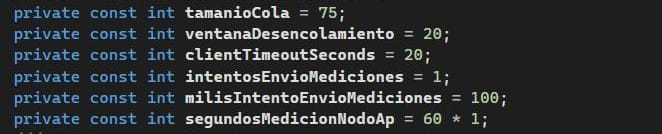
\includegraphics[width=1\linewidth]{Figures//Firmware/configuracion_tuneada.png}
    \caption{Configuración del Nodo AP óptima para red móvil 4G.}
    \label{fig:enter-label}
\end{figure}

Con ello se consiguió una tasa de error menor al 1\%, es decir, de cada 100 mensajes recibidos, menos de 1 no llegó al servidor, para una tasa de recepción de 1 paquete por segundo, durante 8 horas.

Para una tasa mayor a 1 paquete cada 10 segundos, la tasa de error fue de 0\% durante el mismo período.

En conclusión, el sistema es muy estable para manejar una tasa de 1 mensaje LoRa cada 10 segundos, o 360 Nodos Sensores enviando mediciones cada 1 hora (asumiendo que en esa ventana de tiempo se distribuyen uniformemente, de forma de no saturar la cola).

%----------------------------------------------------------------------------------------
%	SUBSECTION - PRUEBAS FUNCIONALES DEL PORTAL WEB
%----------------------------------------------------------------------------------------
\subsection{Pruebas funcionales del portal web}
\label{sec:pruebasPW}

\subsubsection{Visualización de datos en tiempo real}

Se implementaron funcionalidades para la visualización de datos en tiempo real, priorizando la representación precisa y clara de las mediciones de temperatura y humedad registradas por los sensores instalados en las composteras. El objetivo fue asegurar que los datos capturados por los sensores fueran transmitidos y visualizados de manera fluida y sin interrupciones en el portal web.

\subsubsection{Banco de pruebas}
Para estas pruebas se utilizó el siguiente entorno:
\begin{itemize}
    \item Simulación de nodos sensores que envían datos de temperatura y humedad.
    \item Servidor backend recibiendo y procesando los datos enviados.
    \item Interfaz backoffice Grafana para visualizar los datos en tiempo real.
\end{itemize}

Se cargaron diferentes conjuntos de datos en el backend, simulando las variaciones de temperatura y humedad propias de una compostera en funcionamiento. Para las pruebas de rendimiento, se generaron escenarios con múltiples nodos y altos volúmenes de datos. 

\subsubsection{Resultados}
El sistema mostró una correcta visualización de los datos, actualizándose en intervalos de tiempo de pocos segundos. No se experimentaron caídas ni errores significativos durante la transmisión de los datos entre nodos y portal web.

\subsubsection{Acceso al historial de datos}

Se verificó la correcta visualización de datos históricos en el \textit{backoffice}, permitiendo a los administradores consultar y analizar mediciones pasadas de temperatura y humedad, así como posibles errores que se hubieran ocasionado. 

\subsubsection{Banco de pruebas}
\begin{itemize}
    \item Simulación de nodos sensores con datos históricos de diferentes días y horas.
    \item Servidor backend recibiendoo y procesando los datos enviados.
    \item Base de datos almacenando los datos históricos. 
    \item Interfaz backoffice Grafana para visualizar los datos.
\end{itemize}

Se cargaron datos históricos almacenados en la base de datos para ser visualizados en el portal web. Se utilizaron los filtros de fechas proporcionados por Grafana para permitir al usuario la búsqueda específica en un rango de tiempo. 

\subsubsection{Resultados}
El acceso al historial de datos se llevó a cabo de manera exitosa, permitiendo al usuario consultar rangos personalizados de fechas, visualizando los gráficos de manera precisa. 

\subsubsection{Gestión de nuevos nodos}

Se evaluó que los usuarios puedan añadir, editar y eliminar nuevos nodos en el sistema de manera eficiente y sin problemas.

\subsubsection{Banco de pruebas}
\begin{itemize}
    \item Servidor backend recibiendo y procesando consultas de un cliente.    
    \item Base de datos almacenando los datos de diferentes nodos. 
\end{itemize}

Se agregaron, editaron y eliminaron nodos y usuarios en el sistema, a través de la API dedicada del portal web. Se verificó que cada nodo estuviera correctamente vinculado con su correspondiente sensor y que la información proporcionada por los sensores se asigne de forma precisa. 

\subsubsection{Resultados}
El sistema mostró los datos asociados a los nodos de manera correcta, reflejando los cambios insertados de manera consistente. 

\subsubsection{Manejo de errores}

El manejo de errores fue una prioridad para asegurar que el sistema se esté comportando de manera adecuada ante posibles fallas y situaciones inesperadas. 

\begin{itemize}
    \item Simulación de nodos sensores que envían datos de temperatura y humedad.
    \item Servidor backend recibiendo y procesando los datos enviados.
    \item Simulación de situaciones de pérdida de conexión y errores en los datos. 
\end{itemize}

Se efectuaron pruebas para simular fallas en la conexión con los sensores y en la transmisión de datos hacia el backend. Se evaluó la capacidad del sistema para denotar de forma clara y visual los errores, y la capacidad de continuar funcionando pese a la interrupción en los datos. 

\subsubsection{Resultados}
El sistema manejó los errores de manera eficaz, mostrando gráficos y logs con los errores encontrados y continuando con las operaciones sin perder la robustez del servicio. 


%----------------------------------------------------------------------------------------
%	SECTION - PRUEBAS INTEGRALES
%----------------------------------------------------------------------------------------
\section{Pruebas integrales}
\label{sec:pruebasInt}
En la siguiente sección se detallan las pruebas integrales del proyecto, las cuales consisten en una prueba de distancia y otra en condiciones reales, ambas realizadas con todas las piezas del proyecto en conjunto en su versión final: un Nodo Access Point, dos Nodos Sensores, y el Portal Web.

Para los Nodos, versión final implica el uso de cajas estancas con sus firmware compilados en modo release (el código fuente compilado sin el overhead de debugging).
Para el Portal Web, versión final es el despliegue del código del frontend y backoffice en su última versión y la base de datos inicializada con la información de los 3 nodos sin ninguna medición.

Las Figuras \ref{fig:nodoap1EstrFinal} y \ref{fig:nodoap2EstrFinal} muestran dos fotos del Nodo Acces Point, el cual consiste en una caja estanca con el regulador del panel solar, un hub USB para conectar el Router 4G Portátil, y por último el PCB del Nodo Access Point. El regulador a su vez está conectado al panel solar y a la batería.

\begin{figure}[H]
	\centering
	\includegraphics[scale=0.20]{Figures/Pruebas/nodoap1.jpeg}
	\caption{Nodo Access Point - Vista interior}
	\label{fig:nodoap1EstrFinal}
\end{figure}

\begin{figure}[H]
	\centering
	\includegraphics[scale=0.25]{Figures/Pruebas/nodoAP2.jpeg}
	\caption{Nodo Access Point - Vista caja cerrada}
	\label{fig:nodoap2EstrFinal}
\end{figure}

A su vez en la Figura \ref{fig:nodoSensor1EstFinal} observa al Nodo Sensor dentro de su respectiva caja estanca, y en la Figura y \ref{fig:nodoSensor2EstFinal} una foto del Nodo con la caja cerrada. En ambas fotos se muestran los sensores enterrados en muestras de compost reales.

\begin{figure}[H]
	\centering
	\includegraphics[scale=0.25]{Figures/Pruebas/nodoSensor2.jpeg}
	\caption{Nodo Sensor - Vista interior}
	\label{fig:nodoSensor1EstFinal}
\end{figure}

\begin{figure}[H]
	\centering
	\includegraphics[scale=0.25]{Figures/Pruebas/nodoSensor1.jpeg}
	\caption{Nodo Sensor - Vista caja cerrada}
	\label{fig:nodoSensor2EstFinal}
\end{figure}

\subsection{Prueba Integral de Distancia}

El objetivo de la prueba fue comprobar el rango máximo de comunicación entre un Nodo Sensor y el Nodo Access Point.

Esta prueba se realizó en el Parque Ferroviario de Colegiales, el cual se eligió por tener la característica de tener un campo de visión mayor a 500 m y por la proximidad para los miembros del presente proyecto, permitiendo hacer ajustes que no se pueden hacer en campo de manera breve.

La prueba consistió en ubicar un Nodo Access Point en un punto fijo, y mover lentamente un Nodo Sensor en linea recta alejándose del Nodo Access Point que envía mediciones cada 5 segundos.  Se determinó la distancia máxima del alcance LoRa en este entorno cuando durante más de 30 segundos se dejaron de recibir mediciones, independientemente de la orientación de las antenas. El resultado fue de aproximadamente 410 metros.

En la Figura \ref{fig:NodoAp-PruebaDistancia} se ve la configuración del Nodo Access Point fuera de su caja estanca para facilitar las mediciones de tensión, y en la captura de la Figura \ref{fig:PruebaDistancia} se ve el resultado de la distancia medida con Google Maps, geolocalizados con el GPS de un celular Android.

\begin{figure}[H]
	\centering
	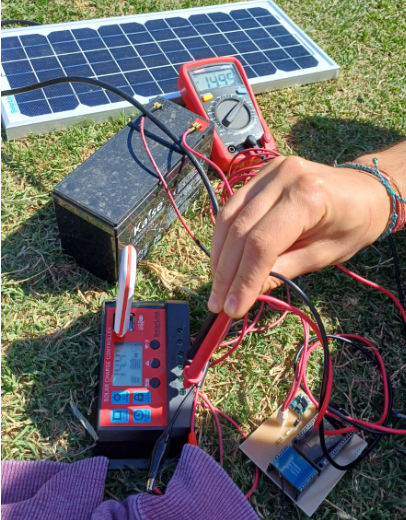
\includegraphics[scale=1]{./Figures/Pruebas/NodoAP-Pruebadistancia.PNG}
	\caption{Nodo Access Point sin su caja estanca.}
	\label{fig:NodoAp-PruebaDistancia}
\end{figure}

\begin{figure}[H]
	\centering
	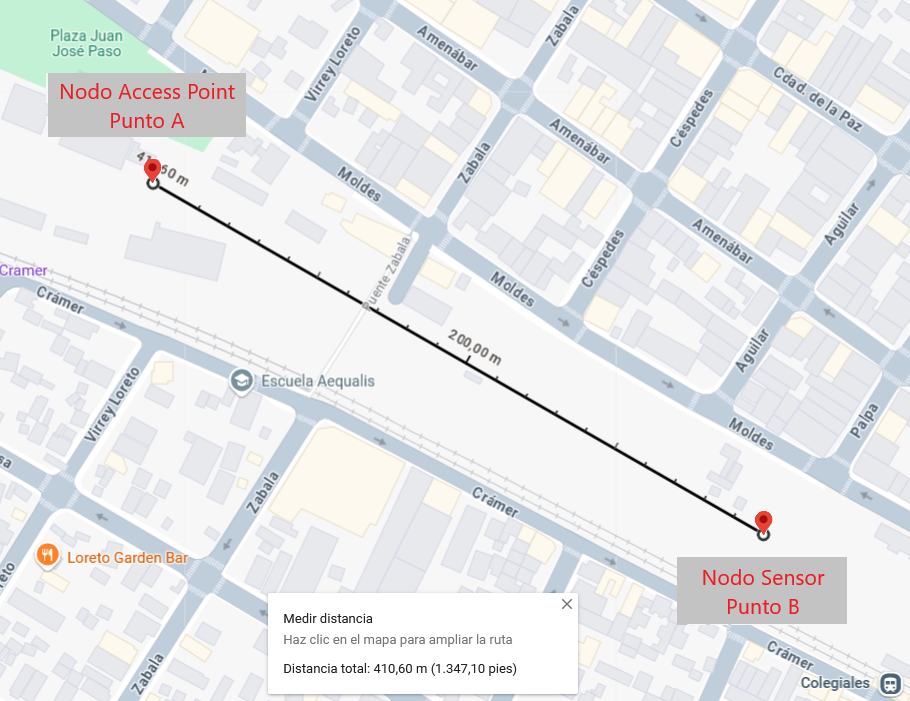
\includegraphics[scale=0.5]{./Figures/Pruebas/prueba_distancia_mapa.png}
	\caption{Visualización geolocalizada de los Nodos de la prueba.}
\label{fig:PruebaDistancia}
\end{figure}

Se consideró la prueba como un caso exitoso dado que a pesar de las condiciones radioeléctricas adversas (rebotes de la señal en los edificios cercanos, obstáculos entre los nodos, etc) los Nodos se comunicaron hasta los 410 metros, lo cual supera los requerimientos del proyecto. Esto quiere decir que en un verdadero campo abierto ideal la distancia máxima debería ser aun mayor.

En la Figura \ref{fig:PruebaDistanciaGrafana} se observan las mediciones que permitieron determinar el rango máximo, como así también el correcto funcionamiento del Nodo Access Point.

\begin{figure}[H]
    \centering
    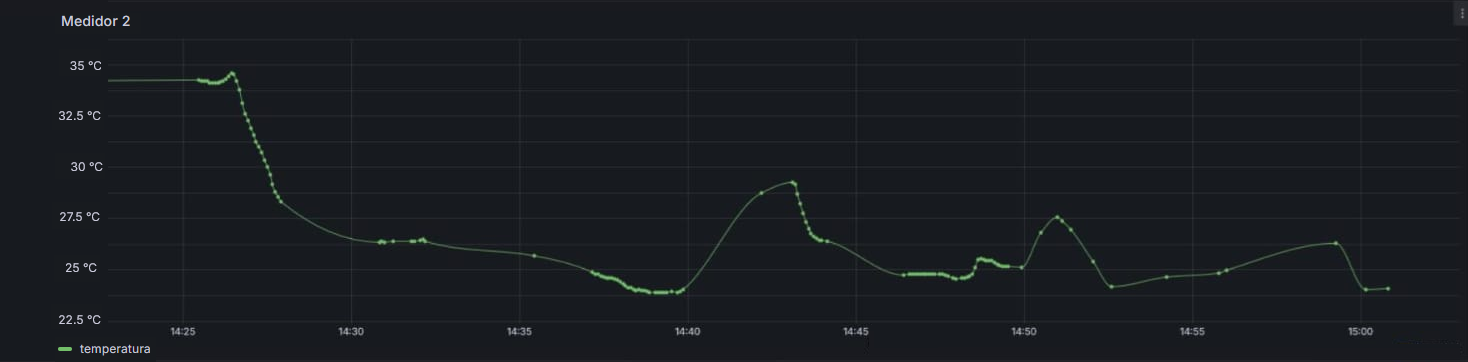
\includegraphics[width=1\linewidth]{Figures/Pruebas/prueba_distancia_grafana.png}
    \caption{Resultados de la prueba integral de distancia en Grafana.}
    \label{fig:PruebaDistanciaGrafana}
\end{figure}

Las distintas densidades de puntos se deben a que durante la prueba se cambiaron constantemente las orientaciones de las antenas. Cuanto menos espaciados están las mediciones mejor fue SNR y calidad de señal, y se observa que las últimas mediciones están muy espaciadas.

\subsection{Prueba Integral en Condiciones Reales}

En esta segunda prueba se verificó el funcionamiento en condiciones reales de los Nodos Sensores y Nodo  Access Point (enviando y recibiendo mediciones cada 1 hora).

Los dos Nodos Sensores se ubicaron en una misma habitación y el Nodo Access Point en un balcón con exposición a la luz solar de manera directa, de forma que el panel solar pueda cargar la batería. (Se entiende que en esta prueba no está maximizado el tiempo de exposición a la luz solar, y por lo tanto el tiempo de carga).

La figura \ref{fig:pruebas_grafana} muestra un tablero de Grafana dividido en dos secciones principales: la mitad superior presenta los gráficos correspondientes al Nodo Sensor número 2, mientras que la mitad inferior visualiza la información recopilada por el Nodo Access Point. Este diseño permite una comparación directa y simultánea de los datos recolectados por ambos nodos, facilitando el monitoreo integral del sistema.
Ambos nodos operaron durante mas de 28 horas sin interrupciones. 
Durante este período, el Nodo Access Point estuvo expuesto a luz solar durante medio día y operó durante otro medio día sin recargar la batería. A partir de estos resultados, se concluye que la capacidad del sistema para operar de manera continua durante más de 24 horas valida la sostenibilidad del ciclo de carga y descarga de la batería, garantizando su funcionamiento eficiente sin interrupciones.

\begin{figure}[H]
    \centering
    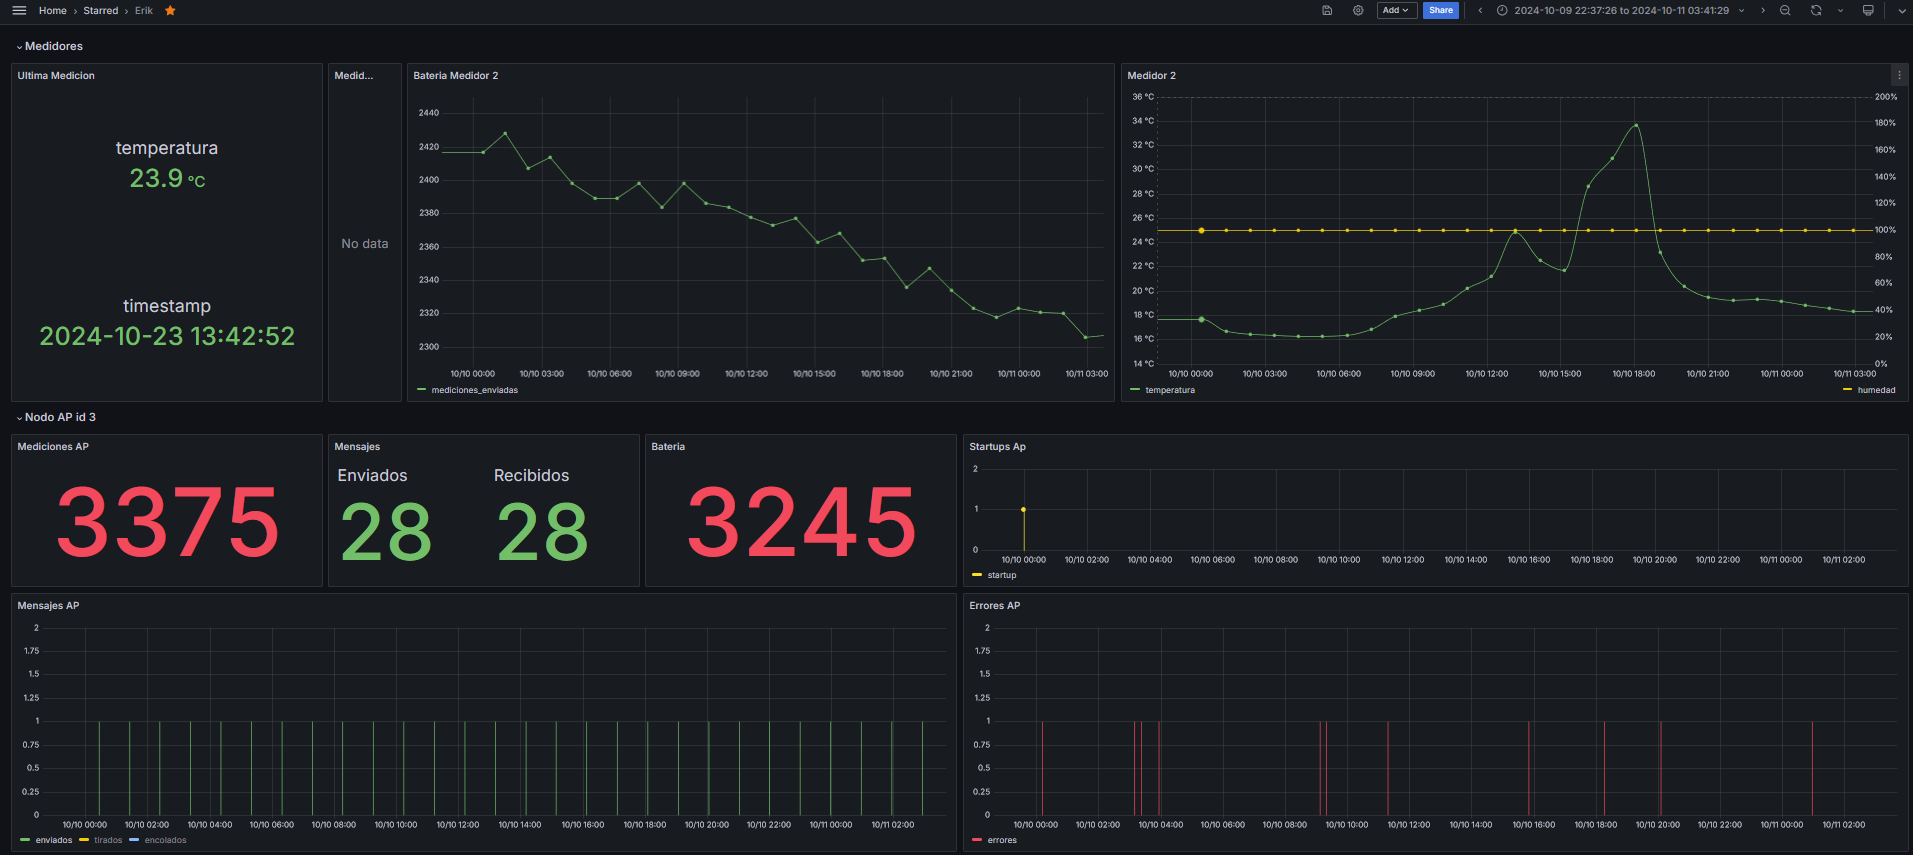
\includegraphics[width=1\linewidth]{Figures/Pruebas/pruebas_grafana.png}
    \caption{Resultados de la prueba integral vistas en Grafana.}
    \label{fig:pruebas_grafana}
\end{figure}

Por un lado, es importante destacar que el nivel de batería del Nodo Sensor 2 no ha sido procesado, por lo que no se presenta en una escala porcentual de 0 a 100, sino como el valor analógico medido.

Por otro lado, el Nodo Access Point demostró estabilidad en el sistema, al recibir y enviar todos los mensajes, así como al registrar una única medición de inicio (startup), lo que indica que, durante toda la prueba, no se produjo ningún reinicio.

Se observa que, en las horas de la tarde, con mayor exposición solar, la temperatura medida aumenta, especialmente entre las 15:00 y las 19:00 horas.

Finalmente, esta prueba reveló que, en un compost muy húmedo, el sensor alcanza una saturación y no muestra variaciones significativas durante períodos prolongados.
 
% Chapter Template

\chapter{Conclusiones} % Main chapter title

\label{Chapter6} % Change X to a consecutive number; for referencing this chapter elsewhere, use \ref{ChapterX}


%----------------------------------------------------------------------------------------

%----------------------------------------------------------------------------------------
%	SECTION 1
%----------------------------------------------------------------------------------------

\section{Conclusiones generales }

El trabajo profesional SmartCompost se diseñó con el propósito de desarrollar una solución automatizada y eficiente para el monitoreo de compost orgánico, centrándose en los parámetros clave de temperatura y humedad. Durante las etapas de diseño y prueba, se trabajó minuciosamente en el cumplimiento de los requerimientos funcionales y no funcionales, con el objetivo de crear un sistema que no solo proporcione lecturas precisas y en tiempo real de las variables monitoreadas, sino que también sea autónomo, escalable, robusto y adaptable a una variedad de entornos operativos.

A continuación, se describen en detalle los logros obtenidos como resultado de la implementación.

El monitoreo continuo de la temperatura y humedad en el compost es un aspecto crucial del proyecto, ya que permite observar los cambios que ocurren durante las distintas etapas del compostaje y ajustar de forma eficiente distintos parámetros para minimizar el tiempo total del proceso. 
Actualmente, esta tarea se realiza manualmente en muchos casos, lo cual puede resultar tedioso, ineficiente y propenso a errores. Con esta solución se automatiza este proceso, proporcionando datos en tiempo real y registrándolos en una base de datos centralizada. Esto permite a los usuarios contar con información fiable y actualizada para optimizar las condiciones de compostaje y obtener un compost de mayor calidad en menos tiempo, como también tener un registro histórico.

Uno de los aspectos centrales del proyecto es la autonomía energética que dispone el Nodo AP. Se diseñó para minimizar la intervención humana y reducir los costos asociados con la alimentación eléctrica en zonas remotas o entornos al aire libre. Por ello el Nodo AP tiene en su diseño un sistema de alimentación basado en baterías y paneles solares. Las pruebas realizadas para verificar la duración de las baterías han sido satisfactorias, lo que garantiza que el proyecto pueda operar de manera continua y sin interrupciones en su totalidad, incluso en condiciones ambientales cambiantes. Esta característica es esencial para la sostenibilidad y eficiencia ya que permite un monitoreo constante sin la preocupación de fallos por falta de energía.

En cuanto a la conectividad y transmisión de datos, el diseño del proyecto aportó una gran flexibilidad  en la integración de diferentes tecnologías de comunicación. Se ha comprobado la eficiencia de la transmisión de datos entre los nodos sensores y el Nodo Access Point. La comunicación, implementada mediante protocolos como LoRa y Wi-Fi, garantiza la transmisión estable y eficiente de los datos. Esta funcionalidad ha sido validada a través de pruebas exhaustivas, demostrando la capacidad del sistema para procesar una medición por nodo por segundo de manera continua y sin interrupciones.

Además, se desarrolló una interfaz de usuario intuitiva y sencilla pensada para facilitar la comprensión de los datos recolectados por los Nodos. Esto permite que cualquier usuario, independientemente de su nivel técnico, pueda interpretar fácilmente la información presentada y tomar decisiones informadas sobre el compost. La interfaz incluye gráficos y mediciones en tiempo real, así como telemetría de cada uno de los Nodos, lo que facilita la supervisión remota y la toma de decisiones en base a datos confiables.

Otro aspecto fundamental del proyecto es su diseño duradero y resistente. Al estar destinado a operar en diversos ambientes, incluyendo exteriores y entornos de compostaje que pueden ser hostiles, el proyecto se diseñó para soportar cambios de temperatura, variaciones de humedad y otros factores externos que puedan afectar su funcionamiento. Cada componente ha sido seleccionado y probado para asegurar su durabilidad, y el sistema en su conjunto ha demostrado ser robusto durante todas las pruebas de campo realizadas. La estructura de los Nodos cuenta con carcasas (cajas estanco) que facilitan su instalación y permiten una fijación segura en distintos entornos, lo que añade una capa de protección y facilita su portabilidad y reubicación cuando sea necesario.

Además de los aspectos ya mencionados, la escalabilidad y flexibilidad del proyecto representan una ventaja significativa. El diseño modular y la compatibilidad con protocolos estándar de comunicación permiten que el proyecto pueda ampliarse con facilidad, integrando nuevos sensores o funcionalidades en el futuro sin necesidad de reestructurar la infraestructura existente. Esto no solo permite que el proyecto crezca con las necesidades del usuario, sino que también asegura que la inversión realizada sea sostenible y adaptable a las nuevas demandas que puedan surgir en el manejo de compost a medida que este proceso evoluciona.

Finalmente, la solución se destaca por su mantenibilidad y facilidad de desarrollo tanto del firmware como del hardware, lo cual es crucial para su funcionalidad a largo plazo. La estructura modular del PCB permite que los componentes puedan ser reemplazados o actualizados sin afectar al resto de los elementos, facilitando tanto las tareas de mantenimiento como las futuras actualizaciones del firmware. Este diseño, sumado a la facilidad de transporte y reubicación de los Nodos, garantiza que SmartCompost pueda adaptarse a distintos entornos y escenarios, lo cual lo convierte en una herramienta versátil y práctica para diversos tipos de usuarios y aplicaciones.
Por su parte, el firmware posee una arquitectura también modular orientada a objetos, el cual junto con el kernel implementado, permite una gran reutilización de código para una fácil escalabilidad y bajo mantenimiento.

En conclusión, el proyecto SmartCompost cumple de manera satisfactoria con todos los requisitos planteados y representa una solución innovadora para el monitoreo automatizado de compost. Aunque se encuentra en una fase inicial, ha demostrado ser una herramienta confiable y eficiente para la supervisión continua del compost, mejorando significativamente los métodos manuales actuales. La implementación de este proyecto permite a los usuarios optimizar el proceso de compostaje con un mínimo esfuerzo y de manera sostenible, lo que resulta en un compost de mayor calidad y en una práctica de compostaje más efectiva y respetuosa con el medio ambiente. SmartCompost no solo facilita el monitoreo de compost, sino que también promueve una gestión más inteligente de los recursos orgánicos.

% La idea de esta sección es resaltar cuáles son los principales aportes del trabajo realizado y cómo se podría continuar. Debe ser especialmente breve y concisa. Es buena idea usar un listado para enumerar los logros obtenidos.

% Algunas preguntas que pueden servir para completar este capítulo:

% \begin{itemize}
% \item ¿Cuál es el grado de cumplimiento de los requerimientos?
% \item ¿Cuán fielmente se puedo seguir la planificación original (cronograma incluido)?
% \item ¿Se manifestó algunos de los riesgos identificados en la planificación? ¿Fue efectivo el plan de mitigación? ¿Se debió aplicar alguna otra acción no contemplada previamente?
% \item Si se debieron hacer modificaciones a lo planificado ¿Cuáles fueron las causas y los efectos?
% \item ¿Qué técnicas resultaron útiles para el desarrollo del proyecto y cuáles no tanto?
% \end{itemize}


%----------------------------------------------------------------------------------------
%	SECTION 2
%----------------------------------------------------------------------------------------
\section{Próximos pasos}

% Acá se indica cómo se podría continuar el trabajo más adelante.

Como próximos pasos se considera esencial contactar a un diseñador industrial. La colaboración con un experto en diseño permitirá desarrollar una estructura más profesional y optimizada que no solo mejore la estética y funcionalidad del proyecto, sino que también facilite su integración en diversos entornos y aplicaciones.

Además, se proyecta la incorporación de nuevos sensores para medir parámetros adicionales, como pH o niveles de gases, lo cual enriquecería las capacidades de monitoreo y análisis de los Nodos Sensores. Estas mejoras podrían abrir el mercado a nuevas aplicaciones, como el monitoreo de procesos en la producción de humus de lombriz y la gestión de parámetros críticos en la agricultura. Expandiendo el proyecto a otros sectores, SmartCompost podría convertirse en una solución versátil para diversos tipos de compostaje y prácticas de cultivo, brindando valor a usuarios tanto domésticos como comerciales.

Como parte de la expansión del proyecto, también se planea la creación de un portal de usuarios donde los clientes puedan visualizar sus datos históricos, obtener recomendaciones basadas en sus registros, y recibir alertas y notificaciones personalizadas. Este portal permitirá a los usuarios gestionar sus dispositivos y acceder a información detallada sobre su compost o cultivos, mejorando así la experiencia de usuario y facilitando la adopción de prácticas más sostenibles y efectivas en la gestión de compost y suelos.

 

%----------------------------------------------------------------------------------------
%	CONTENIDO DE LA MEMORIA  - APÉNDICES
%----------------------------------------------------------------------------------------

\appendix % indicativo para indicarle a LaTeX los siguientes "capítulos" son apéndices

% Incluir los apéndices de la memoria como archivos separadas desde la carpeta Appendices
% Descomentar las líneas a medida que se escriben los apéndices

% Appendix A

\chapter{Archivos de configuración} % Main appendix title
\label{AppendixA} % For referencing this appendix elsewhere, use \ref{AppendixA}


\lstdefinelanguage{yaml}{
  keywords={true,false,null,y,n},
  sensitive=false,
  comment=[l]{\#},
  morecomment=[s]{/*}{*/},
  morestring=[b]',
  morestring=[b]",
  literate = 
   *{=}{{{\color{red}=}}}{1}
    {>}{{{\color{red}>}}}{1},
  keywordstyle=\color{blue}\bfseries,
  commentstyle=\color{gray}\itshape,
  stringstyle=\color{orange},
  basicstyle=\ttfamily\small,
  showstringspaces=false
}

\lstset{
    backgroundcolor=\color{lightgray!20}, % Color de fondo
    frame=single, % Cuadro alrededor del código
    breaklines=true, % Ajuste de línea automático
    basicstyle=\ttfamily\footnotesize, % Tamaño y tipo de fuente
    keywordstyle=\color{blue},
    commentstyle=\color{gray},
    stringstyle=\color{orange}
}
\section{Docker Compose}

\begin{lstlisting}[label=cod:dockercompose,caption=Docker Compose del portal Web de Smartcompst.]  
version: '3.8'

services:
  nginx:
    build:
      context: ./nginx
      dockerfile: Dockerfile
    ports:
      - "80:80"
    volumes:
      - ./nginx/smartcompost.conf:/etc/nginx/nginx.conf
      - ./logs/nginx:/var/log/nginx
    depends_on:
      - frontend
      - web
    logging:
      driver: "json-file"
      options:
        max-size: "10m"
        max-file: "3"

  web:
    build:
      context: ./backend
      dockerfile: Dockerfile
    depends_on:
      - db
    environment:
      DB_HOST: db
      DB_PORT: 3306
      DB_USER: XXX #private info
      DB_PASSWORD: XXX #private info
      DB_NAME: XXX #private info
      CONFIG_PATH: /app/config/config.yml
    ports:
      - "8080:8080"
    volumes:
      - ./logs/web:/var/log/web
    logging:
      driver: "json-file"
      options:
        max-size: "10m"
        max-file: "3"

  db:
    image: mysql:8.0
    environment:
      MYSQL_ROOT_PASSWORD: XXX #private info
      MYSQL_DATABASE: XXX #private info
      MYSQL_USER: XXX #private info
      MYSQL_PASSWORD: XXX #private info
    ports:
      - "3307:3306"
    volumes:
      - db-data:/var/lib/mysql
      - ./init.sql:/docker-entrypoint-initdb.d/init.sql
      - ./logs/mysql:/var/log/mysql
    logging:
      driver: "json-file"
      options:
        max-size: "10m"
        max-file: "3"

  frontend:
    build:
      context: ./frontend
      dockerfile: Dockerfile
    env_file: ./frontend/.env.local
    ports:
      - "3000:3000"
    volumes:
      - ./logs/frontend:/var/log/frontend
    logging:
      driver: "json-file"
      options:
        max-size: "10m"
        max-file: "3"

  loki:
    image: grafana/loki:2.8.2
    ports:
      - "3100:3100"
    volumes:
      - loki-data:/var/loki
      - ./loki/loki-config.yml:/etc/loki/loki-config.yml
    command: -config.file=/etc/loki/loki-config.yml
    networks:
      - logging

  promtail:
    image: grafana/promtail:2.8.2
    volumes:
      - ./promtail/promtail-config.yml:/etc/promtail/promtail-config.yml
      - ./logs/nginx:/var/log/nginx
      - ./logs/web:/var/log/web
      - ./logs/mysql:/var/log/mysql
      - ./logs/frontend:/var/log/frontend
      - /var/lib/docker/containers:/var/lib/docker/containers
    command: -config.file=/etc/promtail/promtail-config.yml
    networks:
      - logging

  grafana:
    image: grafana/grafana:latest
    ports:
      - "3001:3000"
    volumes:
      - grafana-data:/var/lib/grafana
    environment:
      GF_SECURITY_ADMIN_PASSWORD: "XXX" #our grafana password
    networks:
      - logging

volumes:
  db-data:
  loki-data:
  grafana-data:

networks:
  logging:
    driver: bridge
\end{lstlisting}

\section{Configuración Nginx}
\begin{lstlisting}[label=cod:nginx-config,caption=Configuración reverse proxy nginx.] 
events {
}
http {
    access_log /var/log/nginx/access.log;
    error_log /var/log/nginx/error.log;

    server {
        listen 80;

        location / {
            proxy_pass http://frontend:3000;
            proxy_set_header Host $host;
            proxy_set_header X-Real-IP $remote_addr;
            proxy_set_header X-Forwarded-For $proxy_add_x_forwarded_for;
        }
    }
}

\end{lstlisting}

\chapter{Código fuente firmwware} % Main appendix title
\label{AppendixB} % For referencing this appendix elsewhere, use \ref{AppendixA}

\lstset{
    language=[Sharp]C, % Configura el lenguaje como C#
    basicstyle=\ttfamily\footnotesize, % Fuente monoespaciada y tamaño de letra pequeño
    keywordstyle=\color{blue}, % Color para palabras clave
    commentstyle=\color{green}, % Color para los comentarios
    stringstyle=\color{red}, % Color para cadenas de texto
    numbers=left, % Números de línea a la izquierda
    numberstyle=\tiny\color{gray}, % Estilo de los números de línea
    stepnumber=1, % Incremento de los números de línea
    breaklines=true, % Cortar las líneas largas automáticamente
    frame=single, % Cuadro alrededor del código
    captionpos=b % Posición de los títulos (b: abajo)
}

\section{Nodo Sensor}

\begin{lstlisting}[caption={Ejemplo de código en C\#}]

using Equipos.DS18B20;
using Equipos.SX127X;
using nanoFramework.Device.OneWire;
using nanoFramework.Hardware.Esp32;
using NanoKernel.Ayudantes;
using NanoKernel.Dominio;
using NanoKernel.DTOs;
using NanoKernel.Hilos;
using NanoKernel.Logging;
using NanoKernel.Nodos;
using System;
using System.Device.Adc;
using System.Device.Gpio;
using System.Threading;

namespace NodoMedidor
{
    public class NodoMedidor : NodoBase
    {
        public override TiposNodo tipoNodo => TiposNodo.MedidorLora;

        private const int segundosSleep = 60*15;

        // -----LORA-----
        private LoRaDevice lora;
        private const double FRECUENCIA = 433e6;

        private const int PIN_MISO = 19;
        private const int PIN_MOSI = 23;
        private const int PIN_CLK = 18;
        private const int PIN_NSS = 5;
        private const int PIN_DIO0 = 25;
        private const int PIN_RESET = 14;
        // ----LED----
        private GpioController gpio;
        private GpioPin led;

        private const int PIN_LED_ONBOARD = 2;
        // ----SENSORES----
        private OneWireHost oneWire;
        private Ds18b20 ds18b20;
        private GpioPin vccSensores;
        private AdcController adc;
        private AdcChannel humedadAdc;
        private AdcChannel bateriaAdcSensor;
        private AdcChannel bateriaAdcAp;

        private const int ONE_WIRE_RX = 16;  
        private const int ONE_WIRE_TX = 17;
        private const int ADC_HUMEDAD = 0;
        private const int ADC_BATERIA = 3;
        private const float ERROR_TEMP = -100;
        
        // ----VARS----
        private MedicionesNodoDto dto;

        private readonly byte[] bufferLora = new byte[LoRaDevice.MAX_LORA_PAYLOAD_BYTES];

        public override void Setup()
        {
            // ----LED----
            gpio = new GpioController();
            led = gpio.OpenPin(PIN_LED_ONBOARD, PinMode.Output);
            // Prendemos el led para avisar que estamos configurando
            led.Write(PinValue.High);   

            // ----LORA----
            Hilo.Intentar(() =>
            {
                lora = new LoRaDevice(
                    pinMISO: PIN_MISO,
                    pinMOSI: PIN_MOSI,
                    pinSCK: PIN_CLK,
                    pinNSS: PIN_NSS,
                    pinDIO0: PIN_DIO0,
                    pinReset: PIN_RESET);
                lora.Iniciar(FRECUENCIA);
            }, "Lora", accionException: () => { lora?.Dispose(); });

            // ----SENSORES----
            adc = new AdcController();
            humedadAdc = adc.OpenChannel(ADC_HUMEDAD);
            bateriaAdcSensor = adc.OpenChannel(ADC_BATERIA);

            Configuration.SetPinFunction(ONE_WIRE_RX, DeviceFunction.COM3_RX);
            Configuration.SetPinFunction(ONE_WIRE_TX, DeviceFunction.COM3_TX);

            ds18b20 = new Ds18b20(new OneWireHost(), null, false, TemperatureResolution.VeryHigh);
            ds18b20.IsAlarmSearchCommandEnabled = false;

            Hilo.Intentar(() =>
            {
                if (!ds18b20.Initialize())
                    throw new Exception("No se pudo conectar al sensor de temperatura");
            }, intentos: 3);

            // ----DTO----
            dto = new MedicionesNodoDto() { serial_number = Config.NumeroSerie };

            // Avisamos que terminamos de configurar
            led.Write(PinValue.Low);  
        }

        public override void Loop(ref bool activo)
        {
            try
            {
                dto.AgregarMedicion(MedirBateria(), TiposMediciones.Bateria);
                dto.AgregarMedicion(MedirTemperatura(), TiposMediciones.Temperatura);
                dto.AgregarMedicion(MedirHumedad(), TiposMediciones.Humedad);
                dto.last_updated = DateTime.UtcNow;

                long length = dto.ToBytes(bufferLora);
                lora.Enviar(bufferLora, 0, (int)length);

                Logger.Debug($"Paquete {dto.last_updated.Ticks} enviado, {length} bytes");
                Blink();
            }
            catch (Exception ex)
            {
                Logger.Log(ex);
            }
            finally
            {
                dto.measurements.Clear();

                LimpiarMemoria();

                lora.ModoSleep();

                Logger.Debug($"Sleep por {segundosSleep}seg");

                aySleep.DeepSleepSegundos(segundosSleep);

                //Thread.Sleep((int)(segundosSleep * 1000));
            }
        }

        private float MedirHumedad()
        {
            
           // La matematica del sensor es la siguiente
           // Vsensor = (analogread/1023)*5
           // y = -5,9732x^3 + 63,948x^2 - 232,8x + 308,98 
        
            int analogValue = humedadAdc.ReadValue();

            float vSensor = (analogValue / 4095f * 3.3f);
            double humidityPercentage = (-5.9732 * vSensor * vSensor * vSensor) + (63.948 * vSensor * vSensor) - 232.8 * vSensor + 308.98;

            return analogValue;
        }

        private float MedirTemperatura()
        {
            if (!ds18b20.TryReadTemperature(out var currentTemperature))
            {
                Logger.Error("Temperatura: Error de lectura!");
                return ERROR_TEMP;
            }
            else
            {
                Logger.Debug($"Temperatura: {currentTemperature.DegreesCelsius.ToString("F")}\u00B0C");
                return (float)currentTemperature.DegreesCelsius;
            }
        }

        private float MedirBateria()
        {
            int analogValue = bateriaAdcSensor.ReadValue();
            float vSensor = analogValue / 4095f * 3.3f;

            // Mapeo de cotas con el ADC
            // y = a x + b
            // 0 = a * 2.52 V + b
            // 100 = a * 3.3 V + b
            // y = 128.21 * x - 323.06
            double bateriaPorcentaje = 128.21 * vSensor - 323.06;
            if (bateriaPorcentaje > 100) bateriaPorcentaje = 100;
            if (bateriaPorcentaje < 0) bateriaPorcentaje = 0;

            Logger.Debug($"Bateria: {bateriaPorcentaje}");
            return analogValue;
        }

        private void Blink(int milis = 100)
        {
#if DEBUG
            led.Write(PinValue.High);
            Thread.Sleep(milis);
            led.Write(PinValue.Low);
#endif
        }
    }
}

\end{lstlisting}

\section{Nodo AP}

\begin{lstlisting}[caption={Ejemplo de código en C\#}]

using Equipos.SX127X;
using NanoKernel.Ayudantes;
using NanoKernel.Comunicacion;
using NanoKernel.Dominio;
using NanoKernel.DTOs;
using NanoKernel.Herramientas.Comunicacion;
using NanoKernel.Herramientas.Medidores;
using NanoKernel.Hilos;
using NanoKernel.Logging;
using NanoKernel.Nodos;
using System;
using System.Collections;
using System.Device.Adc;
using System.Device.Gpio;
using System.IO;
using System.Threading;

namespace NodoAP
{
    public class NodoAP : NodoBase
    {
        public override TiposNodo tipoNodo => TiposNodo.AccessPointLora;

        /// ------------------------------
        /// CONFIGURACION ROUTER MOVIL 4G
        private const int tamanioCola = 75; 
        private const int ventanaDesencolamiento = 20; 
        private const int clientTimeoutSeconds = 20;
        private const int intentosEnvioMediciones = 1; 
        private const int milisIntentoEnvioMediciones = 100;
        private const int segundosMedicionNodoAp = 60 * 1;
        /// ------------------------------
        private SmartCompostClient cliente;
        private GpioPin led;
        private LoRaDevice lora;
        private const int PIN_MISO = 19;
        private const int PIN_MOSI = 23;
        private const int PIN_CLK = 18;
        private const int PIN_NSS = 5;
        private const int PIN_DIO0 = 25;
        private const int PIN_RESET = 14;
        private const double FREQ_LORA = 433e6;
        /// ------------------------------
        private const int ADC_CHANNEL_BATERIA = 3;
        private AdcController adcController;
        private AdcChannel adcBateria;
        /// ------------------------------
        private ConcurrentQueue colaMedicionesNodo = new ConcurrentQueue(tamanioCola);
        private ArrayList mensajesDesencolados = new ArrayList();
        private MedicionesApDto payloadEnvioMediciones = new MedicionesApDto();
        /// ------------------------------
        private MedicionesNodoDto medicionNodo;
        private Medidor medidor;
        private int mensajesMedicionAP = 0;
        private const string M_TIRADOS = "tirados";
        private const string M_RECIBIDOS = "encolados";
        private const string M_ENVIADOS = "enviados";
        private const string ERRORES = "errores";

        public override void Setup()
        {
            /// Configuramos el LED
            var gpio = new GpioController();
            led = gpio.OpenPin(2, PinMode.Output);
            /// Prendemos el led para avisar que estamos configurando
            led.Write(PinValue.High);

            /// Conectamos a internet
            Hilo.Intentar(() =>
            {
                if (ayInternet.ConectarsePorWifi(Config.RouterSSID, Config.RouterPassword) == false)
                {
                    throw new Exception("Fallo la conexion al router");
                }

                string ip = ayInternet.ObtenerIp();
                if (ip == "0.0.0.0")
                    throw new Exception("No se pudo asignar la ip");

                /// IP asignada
                Logger.Log($"Ip asignada: {ip}");

            }, $"Wifi");

            /// Vemos si podemos pingear la api
            bool ping = ayInternet.Ping(Config.SmartCompostHost);
            if (ping == false)
                Logger.Log("NO HAY PING AL SERVIDOR");

            /// Cliente
            cliente = new SmartCompostClient(Config.SmartCompostHost, Config.SmartCompostPort, clientTimeoutSeconds);

            /// Configuramos el Lora
            Hilo.Intentar(() =>
                {
                    lora = new LoRaDevice(
                        pinMISO: PIN_MISO,
                        pinMOSI: PIN_MOSI,
                        pinSCK: PIN_CLK,
                        pinNSS: PIN_NSS,
                        pinDIO0: PIN_DIO0,
                        pinReset: PIN_RESET);
                    lora.Iniciar(FREQ_LORA);
                    lora.ModoRecibir();
                },
                "Lora",
                accionException: () =>
                {
                    lora?.Dispose();
                });

            /// Mediciones del Nodo AP
            medicionNodo = new MedicionesNodoDto();
            medicionNodo.serial_number = Config.NumeroSerie;
            medicionNodo.last_updated = DateTime.UtcNow;

            // Avisamos que nos despertamos
            medicionNodo.AgregarMedicion(1, TiposMediciones.Startup);
            Hilo.Intentar(() => cliente.AddNodeMeasurments(Config.NumeroSerie, medicionNodo), intentos: 3);
            medicionNodo.measurements.Clear();

            // Inicializamos el medidor del Nodo AP
            adcController = new AdcController();
            adcBateria = adcController.OpenChannel(ADC_CHANNEL_BATERIA);
            medidor = new Medidor(segundosMedicionNodoAp * 1000);
            medidor.OnMedicionesEnPeriodoCallback += Medidor_OnMedicionesEnPeriodoCallback;
            medidor.Iniciar();

            // Escuchamos cuando terminamos de configurar
            lora.OnReceive += Device_OnReceive;

            /// Avisamos que terminamos de configurar
            led.Write(PinValue.Low);
        }

        #region RECEPCION DE MENSAJES
        private void Device_OnReceive(object sender, SX127XDevice.OnDataReceivedEventArgs e)
        {
            try
            {
                if (e.Data == null)
                    throw new Exception("Mensaje null recibido");

                Logger.Debug($"{e.Data.Length} bytes recibidos");

                byte[] mensaje = ValidarYProcesarMensaje(e.Data);
                if (mensaje == null)
                {
                    e.Data = null;
                    medidor.Contar(M_TIRADOS);
                    return;
                }

                medidor.Contar(M_RECIBIDOS);

                byte[] mensajeDesbordado = (byte[])colaMedicionesNodo.Enqueue(mensaje);
                if (mensajeDesbordado != null)
                {
                    mensajeDesbordado = null;
                    medidor.Contar(M_TIRADOS);
                    Logger.Debug("Cola mediciones desbordada");
                }
            }
            catch (Exception ex)
            {
                medidor.Contar(ERRORES);
                Logger.Log(ex.Message);
            }
        }

        private byte[] ValidarYProcesarMensaje(byte[] data)
        {
            using (MemoryStream ms = new MemoryStream(data))
            using (BinaryReader br = new BinaryReader(ms))
            {
                var tipoPaquete = (TipoPaqueteEnum)br.ReadByte();
                if (tipoPaquete != TipoPaqueteEnum.MedicionNodo)
                {
                    Logger.Error($"Mensaje {tipoPaquete} no soportado");
                    return null;
                }

                MedicionesNodoDto.SetearTimestamp(data, ms, br);
                return data;
            }
        }
        #endregion

        #region ENVIO DE MENSAJES
        public override void Loop(ref bool activo)
        {
            if (colaMedicionesNodo.IsEmpty())
            {
                /// Si no hay mensajes encolados liberamos el thread
                Thread.Sleep(100);
                return;
            }

            try
            {
                int tamanioCola = colaMedicionesNodo.Count();
                for (int i = 0; i < ventanaDesencolamiento && !colaMedicionesNodo.IsEmpty(); i++)
                {
                    var item = (byte[])colaMedicionesNodo.Dequeue();
                    try
                    {
                        payloadEnvioMediciones.AgregarMediciones(MedicionesNodoDto.FromBytes(item));
                        mensajesDesencolados.Add(item);
                    }
                    catch (Exception ex)
                    {
                        Logger.Log(ex);
                    }
                }

                if (mensajesDesencolados.Count == 0)
                {
                    medidor.Contar(ERRORES);
                    Logger.Error("No se pudo deserealizar nada");
                    return;
                }

                Logger.Debug($"{mensajesDesencolados.Count}/{tamanioCola} mensajes desencolados");

                // Envio del payload
                payloadEnvioMediciones.last_updated = DateTime.UtcNow;
                bool payloadEnviado = Hilo.Intentar(
                    () => cliente.AddApMeasurments(Config.NumeroSerie, payloadEnvioMediciones),
                    nombreIntento: "Envio payload AP",
                    milisIntento: milisIntentoEnvioMediciones,
                    intentos: intentosEnvioMediciones);

                if (payloadEnviado)
                {
                    Blink(100);

                    medidor.Contar(M_ENVIADOS, mensajesDesencolados.Count - mensajesMedicionAP);
                    Logger.Log($"{mensajesDesencolados.Count} mensajes enviados");
                }
                else
                {
                    medidor.Contar(ERRORES);

                    /// Si podemos volvemos a meterlo en la cola, sino los tiro para dejar lugar a nuevos mensajes
                    int indiceReencolado = 0;
                    object obj = null;
                    do
                    {
                        obj = colaMedicionesNodo.Enqueue(mensajesDesencolados[indiceReencolado++]);
                    }
                    while (obj == null && indiceReencolado < mensajesDesencolados.Count);

                    medidor.Contar(M_TIRADOS, mensajesDesencolados.Count - indiceReencolado + 1);
                    Logger.Debug($"{indiceReencolado + 1} mensajes reencolados");
                }
            }
            catch (Exception e)
            {
                medidor.Contar(ERRORES);
                Logger.Log(e);
            }
            finally
            {
                // Limpiamos toda la memoria posible
                mensajesMedicionAP = 0;
                payloadEnvioMediciones.nodes_measurements.Clear();
                mensajesDesencolados.Clear();
                LimpiarMemoria();

                Logger.Debug($"Enviados: {medidor.ContadoTotal(M_ENVIADOS)} | Tirados: {medidor.ContadoTotal(M_TIRADOS)} | Encolados: {colaMedicionesNodo.Count()}");
            }
        }
        #endregion

        #region MEDICIONES AP
        private void Medidor_OnMedicionesEnPeriodoCallback(InstanteMedicion resultado)
        {
            try
            {
                medicionNodo.AgregarMedicion(colaMedicionesNodo.Count(), TiposMediciones.TamanioCola);

                var recibidos = resultado.ContadoEnPeriodo(M_RECIBIDOS);
                if (recibidos > 0)
                    medicionNodo.AgregarMedicion(recibidos, TiposMediciones.MensajesRecibidos);

                var tirados = resultado.ContadoEnPeriodo(M_TIRADOS);
                if (tirados > 0)
                    medicionNodo.AgregarMedicion(tirados, TiposMediciones.MensajesTirados);

                var errores = resultado.ContadoEnPeriodo(ERRORES);
                if (errores > 0)
                    medicionNodo.AgregarMedicion(errores, TiposMediciones.Errores);

                var enviados = resultado.ContadoEnPeriodo(M_ENVIADOS);
                if (enviados > 0)
                    medicionNodo.AgregarMedicion(enviados, TiposMediciones.MensajesEnviados);

                var bateria = MedirBateria();
                if (bateria > 0)
                    medicionNodo.AgregarMedicion(bateria, TiposMediciones.Bateria);

                medicionNodo.last_updated = DateTime.UtcNow;

                colaMedicionesNodo.Enqueue(medicionNodo.ToBytes());
                mensajesMedicionAP++;
                Logger.Debug("Encolando mediciones del Nodo AP");
            }
            catch (Exception ex)
            {
                medidor.Contar(ERRORES);
                Logger.Log(ex);
            }
            finally
            {
                medicionNodo.measurements.Clear();
            }
        }

        private float MedirBateria()
        {
            int analogValue = adcBateria.ReadValue();
            float vSensor = analogValue / 4095f * 3.3f;

            // Cuenta de la bateria, mapeando las cotas con el ADC
            // y = a x + b
            // 0 = a * 2.52 V + b
            // 100 = a * 3.3 V + b
            // y = 128.21 * x - 323.06
            double bateriaPorcentaje = 128.21 * vSensor - 323.06;
            if (bateriaPorcentaje > 100) bateriaPorcentaje = 100;
            if (bateriaPorcentaje < 0) bateriaPorcentaje = 0;

            return analogValue;
        }

        #endregion

        private void Blink(int time)
        {
            led.Write(PinValue.High);
            Thread.Sleep(time);
            led.Write(PinValue.Low);
        }
    }
}

\end{lstlisting}

%----------------------------------------------------------------------------------------
%	BIBLIOGRAPHY
%----------------------------------------------------------------------------------------

\Urlmuskip=0mu plus 1mu\relax
\raggedright
\nocite{*}
\printbibliography[heading=bibintoc]


%----------------------------------------------------------------------------------------

\end{document}  